%! suppress = MissingImport
%%
%% I/O Prelab (c) 2021-22 Christopher A. Bohn
%%
%% Licensed under the Apache License, Version 2.0 (the "License");
%% you may not use this file except in compliance with the License.
%% You may obtain a copy of the License at
%%     http://www.apache.org/licenses/LICENSE-2.0
%% Unless required by applicable law or agreed to in writing, software
%% distributed under the License is distributed on an "AS IS" BASIS,
%% WITHOUT WARRANTIES OR CONDITIONS OF ANY KIND, either express or implied.
%% See the License for the specific language governing permissions and
%% limitations under the License.
%%

%%
%% (c) 2021 Christopher A. Bohn
%%

\documentclass[12pt]{article}

\usepackage{fullpage}
\usepackage{fancyhdr}
\usepackage[procnames]{listings}
\usepackage{hyperref}
\usepackage{textcomp}
\usepackage{bold-extra}
\usepackage[dvipsnames]{xcolor}
\usepackage{etoolbox}


% Customize the semester (or quarter) and the course number

\newcommand{\courseterm}{Spring 2022}
\newcommand{\coursenumber}{CSCE 231}

% Customize how a typical lab will be managed;
% you can always use \renewcommand for one-offs

\newcommand{\runtimeenvironment}{your account on the \textit{csce.unl.edu} Linux server}
\newcommand{\filesource}{Canvas or {\footnotesize$\sim$}cse231 on \textit{csce.unl.edu}}
\newcommand{\filesubmission}{Canvas}

% These are placeholder commands and will be renewed in each lab

\newcommand{\labnumber}{}
\newcommand{\labname}{Lab \labnumber\ Assignment}
\newcommand{\shortlabname}{}
\newcommand{\duedate}{}

% Individual or team effort

\newcommand{\individualeffort}{This is an individual-effort project. You may discuss concepts and syntax with other students, but you may discuss solutions only with the professor and the TAs. Sharing code with or copying code from another student or the internet is prohibited.}
\newcommand{\teameffort}{This is a team-effort project. You may discuss concepts and syntax with other students, but you may discuss solutions only with your assigned partner(s), the professor, and the TAs. Sharing code with or copying code from a student who is not on your team, or from the internet, is prohibited.}
\newcommand{\freecollaboration}{In addition to the professor and the TAs, you may freely seek help on this assignment from other students.}
\newcommand{\collaborationrules}{}

% Do you care about software engineering?

\providebool{allowspaghetticode}

\setbool{allowspaghetticode}{false}

\newcommand{\softwareengineeringfrontmatter}{
    \ifboolexpe{not bool{allowspaghetticode}}{
        \section*{No Spaghetti Code Allowed}
        In the interest of keeping your code readable, you may \textit{not} use
        any \lstinline{goto} statements, nor may you use any \lstinline{break}
        statements to exit from a loop, nor may you have any functions
        \lstinline{return} from within a loop.
    }{}
}

\newcommand{\spaghetticodepenalties}[1]{
    \ifboolexpe{not bool{allowspaghetticode}}{
        \penaltyitem{1}{for each \lstinline{goto} statement, \lstinline{break}
            statement used to exit from a loop, or \lstinline{return} statement
            that occurs within a loop.}
    }{}
}

% You shouldn't need to customize these,
% but you can if you like

\lstset{language=C, tabsize=4, upquote=true, basicstyle=\ttfamily}
\newcommand{\function}[1]{\textbf{\lstinline{#1}}}
\setlength{\headsep}{0.7cm}
\hypersetup{colorlinks=true}

\newcommand{\startdocument}{
    \pagestyle{fancy}
    \fancyhf{}
    \lhead{\coursenumber}
    \chead{\ Lab \labnumber: \labname}
    \rhead{\courseterm}
    \cfoot{\shortlabname-\thepage}

	\begin{document}
	\title{\ Lab \labnumber}
	\author{\labname}
	\date{Due: \duedate}
	\maketitle

    \textit{\collaborationrules}
}

\newcommand{\rubricitem}[2]{\item[\underline{\hspace{1cm}} +#1] #2}
\newcommand{\bonusitem}[2]{\item[\underline{\hspace{1cm}} Bonus +#1] #2}
\newcommand{\penaltyitem}[2]{\item[\underline{\hspace{1cm}} -#1] #2}

%%
%% labs/common/semester.tex
%% (c) 2021-22 Christopher A. Bohn
%%
%% Licensed under the Apache License, Version 2.0 (the "License");
%% you may not use this file except in compliance with the License.
%% You may obtain a copy of the License at
%%     http://www.apache.org/licenses/LICENSE-2.0
%% Unless required by applicable law or agreed to in writing, software
%% distributed under the License is distributed on an "AS IS" BASIS,
%% WITHOUT WARRANTIES OR CONDITIONS OF ANY KIND, either express or implied.
%% See the License for the specific language governing permissions and
%% limitations under the License.
%%


% Customize the semester (or quarter) and the course number

\newcommand{\courseterm}{Fall 2022}
\newcommand{\coursenumber}{CSCE 231}

% Customize how a typical lab will be managed;
% you can always use \renewcommand for one-offs

\newcommand{\runtimeenvironment}{your account on the \textit{csce.unl.edu} Linux server}
\newcommand{\filesource}{Canvas or {\footnotesize$\sim$}cse231 on \textit{csce.unl.edu}}
\newcommand{\filesubmission}{Canvas}

% Customize for the I/O lab hardware

\newcommand{\developmentboard}{Arduino Nano}
%\newcommand{\serialprotocol}{SPI}
\newcommand{\serialprotocol}{I2C}
%\newcommand{\displaymodule}{MAX7219digits}
%\newcommand{\displaymodule}{MAX7219matrix}
\newcommand{\displaymodule}{LCD1602}

\setbool{usedisplayfont}{true}

\newcommand{\obtaininghardware}{
    The EE Shop has prepared ``class kits'' for CSCE 231; your class kit costs \$30.
    The EE Shop is located at 122 Scott Engineering Center and is open M-F 7am-4pm. You do not need an appointment.
    You may pay at the window with cash, with a personal check, or with your NCard.
    The EE shop does \textit{not} accept credit cards.
}

% Update to reflect the CS2 course(s) at your institute

\newcommand{\cstwo}{CSCE~156, RAIK~184H, or SOFT~161}

% Do you care about software engineering?

\setbool{allowspaghetticode}{false}

% Which assignments are you using this semester, and when are they due?

\newcommand{\pokerlabnumber}{1}
\newcommand{\pokerlabcollaboration}{
    Sections~\ref{sec:connecting}, \ref{sec:terminology}, \ref{sec:gettingstarted}, \ref{subsec:typesofpokerhands}, and~\ref{subsec:studythecode}: \freecollaboration
    Sections~\ref{sec:completingcard} and~\ref{subsec:completepoker}: \individualeffort
}
\newcommand{\pokerlabdue}{Week of August 29, before the start of your lab section}

\newcommand{\keyboardlabnumber}{2}
\newcommand{\keyboardlabcollaboration}{\individualeffort}
\newcommand{\keyboardlabdue}{Week of January 31, before the start of your lab section}

\newcommand{\pointerlabnumber}{3}
\newcommand{\pointerlabcollaboration}{\individualeffort}
\newcommand{\pointerlabdue}{Week of February 7, before the start of your lab section}

\newcommand{\integerlabnumber}{4}
\newcommand{\integerlabcollaboration}{\individualeffort}
\newcommand{\integerlabdue}{Week of February 14, before the start of your lab section}

\newcommand{\floatlabnumber}{5}
\newcommand{\floatlabcollaboration}{\individualeffort}
\newcommand{\floatlabdue}{soon}

\newcommand{\addressinglabnumber}{6}
\newcommand{\addressinglabcollaboration}{\individualeffort}
\newcommand{\addressinglabdue}{Week of February 28, before the start of your lab section}

%bomblab was 7
%attacklab was 8

\newcommand{\pollinglabnumber}{9}
\newcommand{\pollinglabcollaboration}{\individualeffort}
\newcommand{\pollinglabdue}{Week of April 11, before the start of your lab section}
\newcommand{\pollinglabenvironment}{your \developmentboard-based class hardware kit}

\newcommand{\ioprelabnumber}{\pollinglabnumber-prelab}
\newcommand{\ioprelabcollaboration}{\freecollaboration}
\newcommand{\ioprelabdue}{Before the start of your lab section on April 5 or 6}

\newcommand{\interruptlabnumber}{10}
\newcommand{\interruptlabcollaboration}{\individualeffort}
\newcommand{\interruptlabdue}{Week of April 18, before the start of your lab section}
\newcommand{\interruptlabenvironment}{your \developmentboard-based class hardware kit}

\newcommand{\capstonelab}{ComboLock}    % this will come into play when we generalize capstonelab
\newcommand{\capstonelabnumber}{11}
\newcommand{\capstonelabcollaboration}{\teameffort}
\newcommand{\capstonelabdue}{Week of May 2, Before the start of your lab section\footnote{See Piazza for the due dates of teams with students from different lab sections.}}
\newcommand{\capstonelabenvironment}{your \developmentboard-based class hardware kit}

\newcommand{\memorylabnumber}{12}
\newcommand{\memorylabcollaboration}{This is an individual-effort project. You may discuss the nature of memory technologies and of memory hierarchies with classmates, but you must draw your own conclusions.}
\newcommand{\memorylabdue}{Week of May 2, at the end of your lab section}
\newcommand{\memorylabenvironment}{your \developmentboard-based class hardware kit and your account on the \textit{csce.unl.edu} Linux server}

% Labs not used this semester

\newcommand{\concurrencylabnumber}{XX}
\newcommand{\concurrencylabcollaboration}{\individualeffort}
\newcommand{\concurrencylabdue}{not this semester}

\newcommand{\ssbcwarmupnumber}{XX}
\newcommand{\ssbcwarmupcollaboration}{\freecollaboration}
\newcommand{\ssbcwarmupdue}{not this semester}

\newcommand{\ssbcpollingnumber}{XX}
\newcommand{\ssbcpollingcollaboration}{\individualeffort}
\newcommand{\ssbcpollingdue}{not this semester}

\newcommand{\ssbcinterruptnumber}{XX}
\newcommand{\ssbcinterruptcollaboration}{\individualeffort}
\newcommand{\ssbcinterruptdue}{not this semester}

%! suppress = NonMatchingIf

% Text expansion

\newcommand{\power}{power~({\color{red}\textbf{+}}) rail}
\newcommand{\ground}{ground~({\color{blue}\textbf{--}}) rail}
\newcounter{checkpoint}
\newcommand{\checkpoint}[1]{
    \stepcounter{checkpoint}\vspace{1cm}
    \textbf{\textsc{CheckPoint}~\thecheckpoint:}
    Before proceeding further, have a TA or a classmate verify that you have correctly #1.
    Update \textit{checkpoints.txt} file to indicate who checked your work and when they did so.
    \vspace{1cm}
}
\newcommand{\disconnect}{\textbf{Before proceeding further, disconnect the USB cable from the \developmentboard.}}
\newcommand{\rainbow}{male-to-male rainbow cable}
\newcommand{\prepunch}[1]{
    \textit{If you are using a breadboard template} then use a jumper wire's lead to pre-punch holes into contact points #1.
}


% Customization variables

\newcommand{\microcontroller}{}
\newcommand{\formfactor}{}
\providebool{fivevolt}
\providebool{hasnand}

\ifdefstring{\developmentboard}{Arduino Nano}{
    \renewcommand{\microcontroller}{ATmega328P}
    \renewcommand{\formfactor}{nano}
}{}

\ifdefstring{\microcontroller}{ATmega328P}{
    \setbool{fivevolt}{true}
    \setbool{hasnand}{true}
}{}

%! suppress = NonMatchingIf

\newcommand{\mcupin}[1]{\texttt{#1}}
\newcommand{\controlrow}[1]{\pgfmathparse{\controlsstartat+#1}\pgfmathprintnumber{\pgfmathresult}}

\newcommand{\mculeftswitch}{??}
\newcommand{\mculeftswitchpoint}{??}
\newcommand{\mculeftswitchx}{??}
\newcommand{\mculeftswitchy}{??}
\newcommand{\mcurightswitch}{??}
\newcommand{\mcurightswitchpoint}{??}
\newcommand{\mcurightswitchx}{??}
\newcommand{\mcurightswitchy}{??}
\ifdefstring{\formfactor}{nano}{
    \newcommand{\mcux}{1}
    \newcommand{\mcuy}{3}
    \newcommand{\mcuwidth}{15}
    \newcommand{\mcuupperrow}{g1--g15}
    \newcommand{\mculowerrow}{c1--c15}
    \newcommand{\mcufivevolt}{c12}
    \newcommand{\mcufivevoltcontactpoint}{a12}
    \newcommand{\mcuupperground}{g12}
    \newcommand{\mcuuppergroundcontactpoint}{j12}
    \newcommand{\mculowererground}{c14}
    \newcommand{\mculowergroundcontactpoint}{a14}
    \newcommand{\mcubuttonnand}{\mcupin{D2}}
    \newcommand{\mcubuttonnandpoint}{j11}
    \newcommand{\mcukeypadnand}{\mcupin{D3}}
    \newcommand{\mcukeypadnandpoint}{j10}
    \newcommand{\mcukeypadrowone}{\mcupin{D4}}
    \newcommand{\mcukeypadrowonepoint}{j9}
    \newcommand{\mcukeypadrowonex}{9}
    \newcommand{\mcukeypadrowoney}{12}
    \newcommand{\mcukeypadrowfour}{\mcupin{D5}}
    \newcommand{\mcukeypadrowfourpoint}{j8}
    \newcommand{\mcukeypadrowfourx}{8}
    \newcommand{\mcukeypadrowfoury}{12}
    \newcommand{\mcukeypadrowseven}{\mcupin{D6}}
    \newcommand{\mcukeypadrowsevenpoint}{j7}
    \newcommand{\mcukeypadrowsevenx}{7}
    \newcommand{\mcukeypadrowseveny}{12}
    \newcommand{\mcukeypadrowstar}{\mcupin{D7}}
    \newcommand{\mcukeypadrowstarpoint}{j6}
    \newcommand{\mcukeypadrowstarx}{6}
    \newcommand{\mcukeypadrowstary}{12}
    \newcommand{\mculeftbutton}{\mcupin{D8}}
    \newcommand{\mculeftbuttonpoint}{j5}
    \newcommand{\mculeftbuttonx}{5}
    \newcommand{\mculeftbuttony}{12}
    \newcommand{\mcurightbutton}{\mcupin{D9}}
    \newcommand{\mcurightbuttonpoint}{j4}
    \newcommand{\mcurightbuttonx}{4}
    \newcommand{\mcurightbuttony}{12}
    \newcommand{\mcukeypadcolone}{\mcupin{D14/A0}}
    \newcommand{\mcukeypadcolonepoint}{a4}
    \newcommand{\mcukeypadcolonex}{4}
    \newcommand{\mcukeypadcoloney}{1}
    \newcommand{\mcukeypadcoltwo}{\mcupin{D15/A1}}
    \newcommand{\mcukeypadcoltwopoint}{a5}
    \newcommand{\mcukeypadcoltwox}{5}
    \newcommand{\mcukeypadcoltwoy}{1}
    \newcommand{\mcukeypadcolthree}{\mcupin{D16/A2}}
    \newcommand{\mcukeypadcolthreepoint}{a6}
    \newcommand{\mcukeypadcolthreex}{6}
    \newcommand{\mcukeypadcolthreey}{1}
    \newcommand{\mcukeypadcolA}{\mcupin{D17/A3}}
    \newcommand{\mcukeypadcolApoint}{a7}
    \newcommand{\mcukeypadcolAx}{7}
    \newcommand{\mcukeypadcolAy}{1}
    \ifdefstring{\serialprotocol}{I2C}{
        \renewcommand{\mcurightswitch}{\mcupin{D10}}
        \renewcommand{\mcurightswitchpoint}{j3}
        \renewcommand{\mcurightswitchx}{3}
        \renewcommand{\mcurightswitchy}{12}
        \renewcommand{\mculeftswitch}{\mcupin{D11}}
        \renewcommand{\mculeftswitchpoint}{j2}
        \renewcommand{\mculeftswitchx}{2}
        \renewcommand{\mculeftswitchy}{12}
        \newcommand{\mcuscl}{\mcupin{D19/A5}}
        \newcommand{\mcusclpoint}{a9}
        \newcommand{\mcusda}{\mcupin{D18/A4}}
        \newcommand{\mcusdapoint}{a8}
    }{}
    \ifdefstring{\serialprotocol}{SPI}{
        \renewcommand{\mculeftswitch}{\mcupin{D18/A4}}
        \renewcommand{\mculeftswitchpoint}{a8}
        \renewcommand{\mculeftswitchx}{8}
        \renewcommand{\mculeftswitchy}{1}
        \renewcommand{\mcurightswitch}{\mcupin{D19/A5}}
        \renewcommand{\mcurightswitchpoint}{a9}
        \renewcommand{\mcurightswitchx}{9}
        \renewcommand{\mcurightswitchy}{1}
        \newcommand{\mcusck}{\mcupin{D13}}
        \newcommand{\mcusckpoint}{a1}
        \newcommand{\mcucs}{\mcupin{D10}}
        \newcommand{\mcucspoint}{j3}
        \newcommand{\mcucopi}{\mcupin{11}}
        \newcommand{\mcucopipoint}{j2}
    }{}
    
    \newcommand{\resistorcontactpointone}{i1}
    \newcommand{\resistorcontactpointtwo}{i16}
    \newcommand{\ledanodecontactpoint}{j16}
    \newcommand{\ledpin}{\mcupin{D12}}
}{}

\newcommand{\controlsstartat}{\mcux+\mcuwidth+2}
\newcommand{\leftbuttontarget}{\mculeftbuttonpoint}
\newcommand{\rightbuttontarget}{\mcurightbuttonpoint}
\newcommand{\mculeftbuttonfrom}{e\controlrow{11}}
\newcommand{\mcurightbuttonfrom}{e\controlrow{15}}
\newcommand{\keypadrowtargetcol}{j}
\newcommand{\keypadrowtargetrowstart}{\mcukeypadrowonex}
\newcommand{\mcukeypadrowfromcol}{h}
\newcommand{\mcukeypadrowfromcontrolrowstart}{0}
\newcommand{\keypadcolumntargetcol}{a}
\newcommand{\keypadcolumnonetargetrow}{\mcukeypadcolonex}
\newcommand{\keypadcolumntwotargetrow}{\mcukeypadcoltwox}
\newcommand{\keypadcolumnthreetargetrow}{\mcukeypadcolthreex}
\newcommand{\keypadcolumnAtargetrow}{\mcukeypadcolAx}
\newcommand{\mcukeypadcolumnfromcol}{h}
\newcommand{\mcukeypadcolumnonefromrow}{\controlrow{4}}
\newcommand{\mcukeypadcolumntwofromrow}{\controlrow{5}}
\newcommand{\mcukeypadcolumnthreefromrow}{\controlrow{6}}
\newcommand{\mcukeypadcolumnAfromrow}{\controlrow{7}}
\ifbool{hasnand}{
    \newcommand{\nandx}{\mcux+\mcuwidth+2}
    \newcommand{\nandy}{5}
    \newcommand{\nandupperrow}{f24--f18}
    \newcommand{\nandlowerrow}{e18--e24}
    \newcommand{\nanduppernc}{g21--j21}
    \newcommand{\nandlowernc}{a20--d20}
    \newcommand{\nandvcc}{j18}
    \newcommand{\nandground}{a24}
    \newcommand{\nandgroundwire}{\drawlabelledtarget{\nandx+6}{1}{1}{\mculowergroundcontactpoint}\drawlabelledtarget{\mcux+13}{1}{1}{\nandground}}
    \newcommand{\nandupperc}{j20}
    \newcommand{\nandupperd}{j19}
    \newcommand{\nanduppery}{i24}
    \newcommand{\buttonnandoutput}{\drawlabelledtarget{\nandx+6}{11}{1}{\mcubuttonnandpoint}\drawlabelledtarget{\mcux+10}{12}{4}{\nanduppery}}
    \newcommand{\nandlowery}{c23}
    \newcommand{\keypadnandoutput}{\drawlabelledtarget{\nandx+5}{3}{1}{\mcukeypadnandpoint}\drawlabelledtarget{\mcux+9}{12}{4}{\nandlowery}}
    \newcommand{\nandupperain}{i23}
    \newcommand{\nandupperaout}{h23}
    \newcommand{\nandupperbin}{i22}
    \newcommand{\nandupperbout}{h22}
    \newcommand{\nandlowerain}{c18}
    \newcommand{\nandloweraout}{b18}
    \newcommand{\nandlowerbin}{c19}
    \newcommand{\nandlowerbout}{b19}
    \newcommand{\nandlowercin}{c21}
    \newcommand{\nandlowercout}{b21}
    \newcommand{\nandlowerdin}{c22}
    \newcommand{\nandlowerdout}{b22}
    \renewcommand{\controlsstartat}{\nandx+8}
    \renewcommand{\leftbuttontarget}{\nandupperbin}
    \renewcommand{\rightbuttontarget}{\nandupperain}
    \renewcommand{\mculeftbuttonfrom}{\nandupperbout}
    \renewcommand{\mcurightbuttonfrom}{\nandupperaout}
    \renewcommand{\keypadcolumntargetcol}{c}
    \renewcommand{\keypadcolumnonetargetrow}{\controlrow{-8}}
    \renewcommand{\keypadcolumntwotargetrow}{\controlrow{-7}}
    \renewcommand{\keypadcolumnthreetargetrow}{\controlrow{-5}}
    \renewcommand{\keypadcolumnAtargetrow}{\controlrow{-4}}
    \renewcommand{\mcukeypadcolumnfromcol}{b}
    \renewcommand{\mcukeypadcolumnonefromrow}{\keypadcolumnonetargetrow}
    \renewcommand{\mcukeypadcolumntwofromrow}{\keypadcolumntwotargetrow}
    \renewcommand{\mcukeypadcolumnthreefromrow}{\keypadcolumnthreetargetrow}
    \renewcommand{\mcukeypadcolumnAfromrow}{\keypadcolumnAtargetrow}
}{}

\newcommand{\leftswitchwire}{\drawlabelledtarget{\controlsstartat+1}{5}{1}{\mculeftswitchpoint}\drawlabelledtarget{\mculeftswitchx}{\mculeftswitchy}{1+3*(\mculeftswitchy-1)/11}{e\controlrow{1}}}
\newcommand{\rightswitchwire}{\drawlabelledtarget{\controlsstartat+6}{5}{1}{\mcurightswitchpoint}\drawlabelledtarget{\mcurightswitchx}{\mcurightswitchy}{1+3*(\mcurightswitchy-1)/11}{e\controlrow{6}}}

\newcommand{\leftbuttonwire}{
    \drawlabelledtarget{\controlsstartat+11}{5}{1}{\leftbuttontarget}
    \drawlabelledtarget{\mculeftbuttonx}{\mculeftbuttony}{4}{\mculeftbuttonfrom}
    \ifbool{hasnand}{
        \drawlabelledtarget{\nandx+4}{\nandy+6}{1}{e\controlrow{11}}
        \drawlabelledtarget{\nandx+4}{\nandy+5}{4}{\mculeftbuttonpoint}
    }{}
}
\newcommand{\rightbuttonwire}{
    \drawlabelledtarget{\controlsstartat+15}{5}{1}{\rightbuttontarget}
    \drawlabelledtarget{\mcurightbuttonx}{\mcurightbuttony}{4}{\mcurightbuttonfrom}
    \ifbool{hasnand}{
        \drawlabelledtarget{\nandx+5}{\nandy+6}{1}{e\controlrow{15}}
        \drawlabelledtarget{\nandx+5}{\nandy+5}{4}{\mcurightbuttonpoint}
    }{}
}

\newcommand{\keypadrowwires}{
    \foreach \x in {0,1,2,3} {
        \drawlabelledtarget{\mcukeypadrowonex-\x}{\mcukeypadrowoney}{4}{\mcukeypadrowfromcol\controlrow{\mcukeypadrowfromcontrolrowstart+\x}}
        \drawlabelledtarget{\controlsstartat+\x}{10}{4}{\keypadrowtargetcol\pgfmathparse{\keypadrowtargetrowstart-\x}\pgfmathprintnumber{\pgfmathresult}}
    }
}

\newcommand{\keypadcolumnwires}{
    \drawlabelledtarget{\controlsstartat+4}{10}{4}{\keypadcolumntargetcol\keypadcolumnonetargetrow}
    \drawlabelledtarget{\controlsstartat+5}{10}{4}{\keypadcolumntargetcol\keypadcolumntwotargetrow}
    \drawlabelledtarget{\controlsstartat+6}{10}{4}{\keypadcolumntargetcol\keypadcolumnthreetargetrow}
    \drawlabelledtarget{\controlsstartat+7}{10}{4}{\keypadcolumntargetcol\keypadcolumnAtargetrow}
    \drawlabelledtarget{\mcukeypadcolonex}{\mcukeypadcoloney}{1}{\mcukeypadcolumnfromcol\mcukeypadcolumnonefromrow}
    \drawlabelledtarget{\mcukeypadcoltwox}{\mcukeypadcoltwoy}{1}{\mcukeypadcolumnfromcol\mcukeypadcolumntwofromrow}
    \drawlabelledtarget{\mcukeypadcolthreex}{\mcukeypadcolthreey}{1}{\mcukeypadcolumnfromcol\mcukeypadcolumnthreefromrow}
    \drawlabelledtarget{\mcukeypadcolAx}{\mcukeypadcolAy}{1}{\mcukeypadcolumnfromcol\mcukeypadcolumnAfromrow}
    \ifbool{hasnand}{
        \drawlabelledtarget{\nandx}{2}{4}{a4}
        \drawlabelledtarget{\nandx+1}{2}{4}{a5}
        \drawlabelledtarget{\nandx+3}{2}{4}{a6}
        \drawlabelledtarget{\nandx+4}{2}{4}{a7}
        \drawlabelledtarget{\nandx}{3}{1}{h\controlrow{4}}
        \drawlabelledtarget{\nandx+1}{3}{1}{h\controlrow{5}}
        \drawlabelledtarget{\nandx+3}{3}{1}{h\controlrow{6}}
        \drawlabelledtarget{\nandx+4}{3}{1}{h\controlrow{7}}
    }{}
}

%! suppress = NonMatchingIf
\newcommand{\namerows}[1]{
    \draw (#1,1)  node {\tiny{a}};
    \draw (#1,2)  node {\tiny{b}};
    \draw (#1,3)  node {\tiny{c}};
    \draw (#1,4)  node {\tiny{d}};
    \draw (#1,5)  node {\tiny{e}};
    \draw (#1,8)  node {\tiny{f}};
    \draw (#1,9)  node {\tiny{g}};
    \draw (#1,10) node {\tiny{h}};
    \draw (#1,11) node {\tiny{i}};
    \draw (#1,12) node {\tiny{j}};
}

\newcommand{\drawic}[4]{
    \draw[gray,very thin] (#1,#2) +(-.4,-.4) rectangle +(#3-.6,3.4);
    \draw[gray,very thin]  (#1,#2) +(-.4,1) arc [start angle=-90, end angle=90, radius=.5];
    \draw[black] (#1,#2) +(-.2,-.2) rectangle +(#3-.8,.2);
    \draw[black] (#1,#2) +(-.2,2.8) rectangle +(#3-.8,3.2);
    \draw (#1,#2) +(#3*.5-.5,1.5) node {\centering \tiny{#4}};
}

\newcommand{\drawtarget}[2]{\draw[black] (#1,#2) circle (2pt);}

%! suppress = MissingImport
\newcommand{\drawlabelledtarget}[4]{
    \drawtarget{#1}{#2}
    \ifnumequal{#3}{1}{\draw (#1,#2) +( 4pt, 4pt) node {\rotatebox{ 45}{\scalebox{.4}{#4}}};}{}
    \ifnumequal{#3}{2}{\draw (#1,#2) +(-4pt, 4pt) node {\rotatebox{-45}{\scalebox{.4}{#4}}};}{}
    \ifnumequal{#3}{3}{\draw (#1,#2) +(-4pt,-4pt) node {\rotatebox{ 45}{\scalebox{.4}{#4}}};}{}
    \ifnumequal{#3}{4}{\draw (#1,#2) +( 4pt,-4pt) node {\rotatebox{-45}{\scalebox{.4}{#4}}};}{}
}

\newcommand{\drawx}[2]{
    \draw (#1,#2) +(-.2,-.2) -- +(.2,.2);
    \draw (#1,#2) +(-.2,.2) -- +(.2,-.2);
}

\newcommand{\drawnanopower}[1]{
    \drawtarget{#1+11}{12}
    \draw (#1+11,12) -- (#1+11,20) -- (9,20) node[ground] {\tiny{upper ground rail}};
    \ifbool{fivevolt}{
        \drawtarget{#1+11}{1}
        \draw (#1+11,1) -- (#1+11,-3)
    }{
        \drawtarget{#1+1}{1}
        \draw (#1+1,1) -- (#1+1,-3)
    } -- (-2,-3) -- (-2,17) node[vcc] {\tiny{upper power rail}};
}

\newcommand{\drawnandpower}[1]{
    \foreach \x in {0,1,2} {
        \drawtarget{#1+\x}{12}
        \draw[rounded corners] (#1,12) +(\x,0) -- +(\x,5) -- (#1-.5,17);
    }
    \draw (#1,17) -- (16.5,17);
    \draw (16.5,17) arc [start angle=0, end angle=180, radius=.5];
    \draw (15.5,17) -- (12.5,17);
    \draw (12.5,17) arc [start angle=0, end angle=180, radius=.5];
    \draw (11.5,17) -- (-2,17);
    \nandgroundwire
}

%! suppress = Ellipsis
\newcommand{\drawbreadboard}{
    \foreach \x in {1,2,...,63} {
        \foreach \y in {1,2,...,5} {
            \draw[white,fill=gray] (\x,\y) circle (1pt);
        }
        \foreach \y in {8,9,...,12} {
            \draw[white,fill=gray] (\x,\y) circle (1pt);
        }
        \draw (\x,-.5)  node {\rotatebox{45}{\tiny{$\x$}}};
        \draw (\x,13.5) node {\rotatebox{45}{\tiny{$\x$}}};
    }
    \foreach \x in {5,10,...,60} {
        \draw[gray,very thin] (\x,-.3) -- (\x,.5);
    }
    \drawx{1}{1}
    \drawx{1}{12}
    \drawx{63}{1}
    \drawx{63}{12}
    \namerows{0}
    \namerows{64}
    \namerows{\mcux+\mcuwidth+0.5}
    \namerows{44.5}
}

\newcommand{\drawnano}[3] {
    \draw[gray,very thin] (#1,#2) +(-1.4,-.4) rectangle +(15.4,6.4);
    \draw[black] (#1,#2) +(-.2,-.2)  rectangle +(14.2,.2);
    \draw[black] (#1,#2) +(-.2,5.8)  rectangle +(14.2,6.2);
    \draw (#1,#2) +(7,3.5) node {\centering \tiny{#3}};
    \draw (#1,#2) +(-1.8,3) node {\rotatebox{90}{\centering \tiny{USB}}};
    \drawnanopower{#1}
}

\newcommand{\drawnand}[2]{
    \drawic{#1}{#2}{7}{\ifbool{fivevolt}{74LS20}{74HC20}}
    \drawnandpower{#1}
    \buttonnandoutput
    \keypadnandoutput
}

\newcommand{\drawswitch}[2]{
    \draw[gray,very thin] (#1,#2) +(-.4,-.4) rectangle +(2.4,.4);
    \draw[black] (#1,#2) +(-.2,-.2) rectangle +(2.2,.2);
    \draw (#1,#2) +(1,-.6) node {\centering \tiny{switch}};
}

\newcommand{\drawbutton}[3]{
    \ifnumequal{#3}{2}{
        \draw[gray,very thin] (#1,#2) +(-.25,-1.25) rectangle +(2.25,1.25);
        \draw[black] (#1,#2) +(-.2,-.2) rectangle +(.2,.2);
        \draw[black] (#1,#2) +(1.8,-.2) rectangle +(2.2,.2);
        \draw (#1,#2) +(1,-.6) node {\centering \tiny{button}};
    }{
        \draw[gray,very thin] (#1,#2) +(-.25,.2) rectangle +(2.25,2.8);
        \draw[black] (#1,#2) +(-.2,-.2) rectangle +(.2,.2);
        \draw[black] (#1,#2) +(1.8,-.2) rectangle +(2.2,.2);
        \draw[black] (#1,#2) +(-.2,2.8) rectangle +(.2,3.2);
        \draw[black] (#1,#2) +(1.8,2.8) rectangle +(2.2,3.2);
        \draw (#1,#2) +(1,.6) node {\centering \tiny{button}};
    }
}

\newcommand{\drawkeypad}[2]{
    \draw[gray,very thin] (#1,#2) +(-.4,-.4) rectangle +(7.4,.4);
    \draw[black] (#1,#2) +(-.2,-.2) rectangle +(7.2,.2);
    \draw (#1,#2) +(1.5,.5) node {\centering \tiny{rows}};
    \draw (#1,#2) +(5.5,.6) node {\centering \tiny{cols}};
    \draw (#1,#2) +(3.5,-.6) node {\centering \tiny{keypad}};
}

\newcommand{\drawiiclcd}[2]{
    \draw[gray,very thin] (#1,#2) +(-.4,-.4) rectangle +(15.4,6.4);
    \draw[black] (#1,#2) +(-.2,-.2) rectangle +(15.2,.2);
    \foreach \y in {1.5,2.5,3.5,4.5} {
        \draw[gray,very thin] (#1,#2) +(-2.5,\y) -- +(.5,\y);
    }
    \draw[gray!50,fill=gray!50] (#1,#2) +(15.5,2.4) rectangle +(17,3.6);
    \draw[gray] (#1,#2) +(14.5,2.5) -- +(17,2.5);
    \draw[gray] (#1,#2) +(14.5,3.5) -- +(17,3.5);
    \draw (#1,#2) +(7.5,5.5) node {\centering \tiny{LCD Serial Adapter}};
}

\newcommand{\drawlcdisplay}[2]{
    \draw[gray,very thin] (#1,#2) +(-3,.4) rectangle +(28.4,-13.4);
    \draw[gray,very thin] (#1,#2) +(-1,-1.8) rectangle +(26,-11.4);
    \draw[black] (#1,#2) +(-.2,-.2) rectangle +(15.2,.2);
    \draw (#1,#2) +(8,-12.5) node {\centering \tiny{LCD 2x16-character Display Module}};
}

%TODO: parameterize
\newcommand{\drawledcircuit}{
    \ctikzset{bipoles/resistor/height=0.1}
    \ctikzset{bipoles/resistor/width=0.3}
    \ctikzset{bipoles/diode/height=0.2}
    \ctikzset{bipoles/diode/width=0.2}
    \draw (.8,10.8)   rectangle (1.2,11.2);
    \draw (15.8,10.8) rectangle (16.2,11.2);
    \draw (15.8,11.8) rectangle (16.2,12.2);
    \draw (1,11) -- (1.5,10.5) to[R] (15.5,10.5) -- (16,11);
    \draw (16,12) -- (16,14) to[led] (16,17) -- (16,20) -- (9,20);
}

%TODO: paramterize number of pins
\newcommand{\drawswitches}[1]{
    \foreach \x in {0,5} {
        \drawswitch{#1+\x}{1}
        \drawtarget{#1+\x+1}{5}
        \draw[rounded corners] (#1+\x+1,5) -- ++(1,2-\x/10) -- ++(5-.8*\x,0) -- ++(.5,1+\x/10) -- +(0,12) -- (9,20);
    }
    \leftswitchwire
    \rightswitchwire
}

\newcommand{\drawbuttons}[2]{
    \foreach \x in {0,4} {
        \drawbutton{#1+\x}{1}{#2}
        \drawtarget{#1+\x+2}{5}
        \draw[rounded corners] (#1+\x+2,5) -- +(.5,1) -- +(.5,15) -- (9,20);
    }
    \leftbuttonwire
    \rightbuttonwire
}

%! suppress = Ellipsis
\newcommand{\drawkeypadandtargets}[1]{
    \drawkeypad{#1}{12}
    \keypadrowwires
    \keypadcolumnwires
}

\newcommand{\drawdisplay}[1]{
    \drawiiclcd{#1}{11}
    \drawlcdisplay{#1}{9}
    \drawlabelledtarget{8}{1}{4}{  SDA}
    \drawlabelledtarget{9}{1}{4}{ SCL}
%TODO: paramterize \drawdisplay by display type
%    \drawlabelledtarget{3}{12}{1}{CS}
%    \drawlabelledtarget{2}{12}{1}{ DIN}
%    \drawlabelledtarget{1}{1}{4}{  SCK}
}


\renewcommand{\labnumber}{\ioprelabnumber}
\renewcommand{\labname}{Physical Assembly of Hardware for I/O Labs}
\renewcommand{\shortlabname}{i/o-prelab}
\renewcommand{\collaborationrules}{\ioprelabcollaboration}
\renewcommand{\duedate}{\ioprelabdue}


\pagelayout
\begin{document}
\labidentifier

In the I/O labs, we will use a microcontroller board with some peripherals.
In this prelab, you will assemble the hardware for the I/O labs.

\section{Obtaining the Hardware}                            \obtaininghardware

\section{Inventorying the Hardware} \label{sec:inventory}   %! suppress = NonMatchingIf
\newcommand{\devboardimage}{}
\newcommand{\nandchipitem}{}
\newcommand{\displaymoduleitem}{}
\newcommand{\fmcableitem}{}

\ifdefstring{\developmentboard}{Arduino Nano}{
    \renewcommand{\devboardimage}{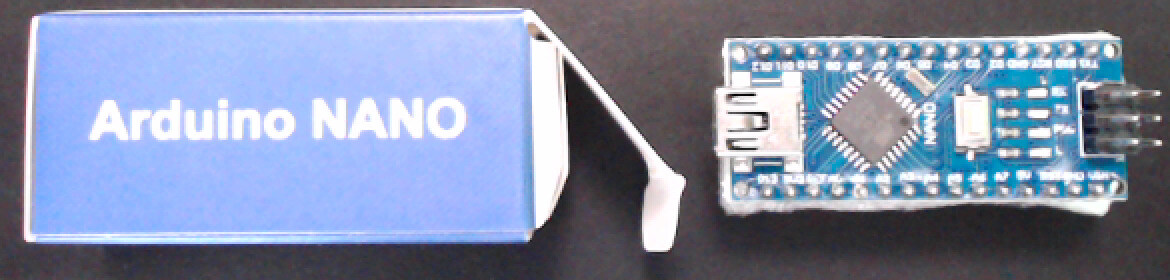
\includegraphics[height=2cm]{inventory/nano}}
    \renewcommand{\nandchipitem}{\item One (1) 74LS20\footnote{Any 74x20 or 54x20 integrated circuit is acceptable.} dual 4-input NAND integrated circuit \\ 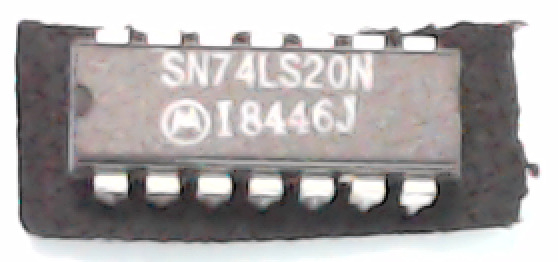
\includegraphics[height=2cm]{inventory/nand}}
}{}
\ifdefstring{\displaymodule}{MAX7219digits}{
    \renewcommand{\displaymoduleitem}{\item One (1) 8-digit 7-segment display module \\ 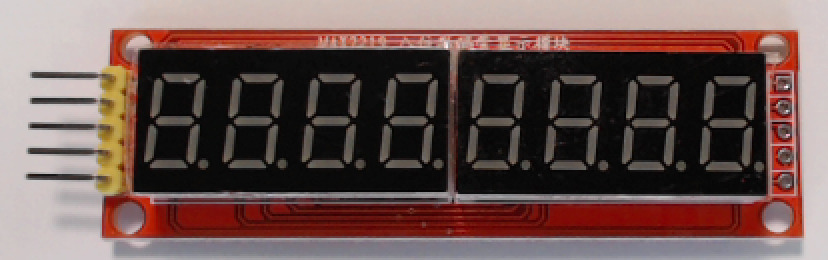
\includegraphics[height=2cm]{inventory/max7219digits}}
    \renewcommand{\fmcableitem}{\item One (1) 5-conductor 20cm ``rainbow'' cable (female-to-male) \\ 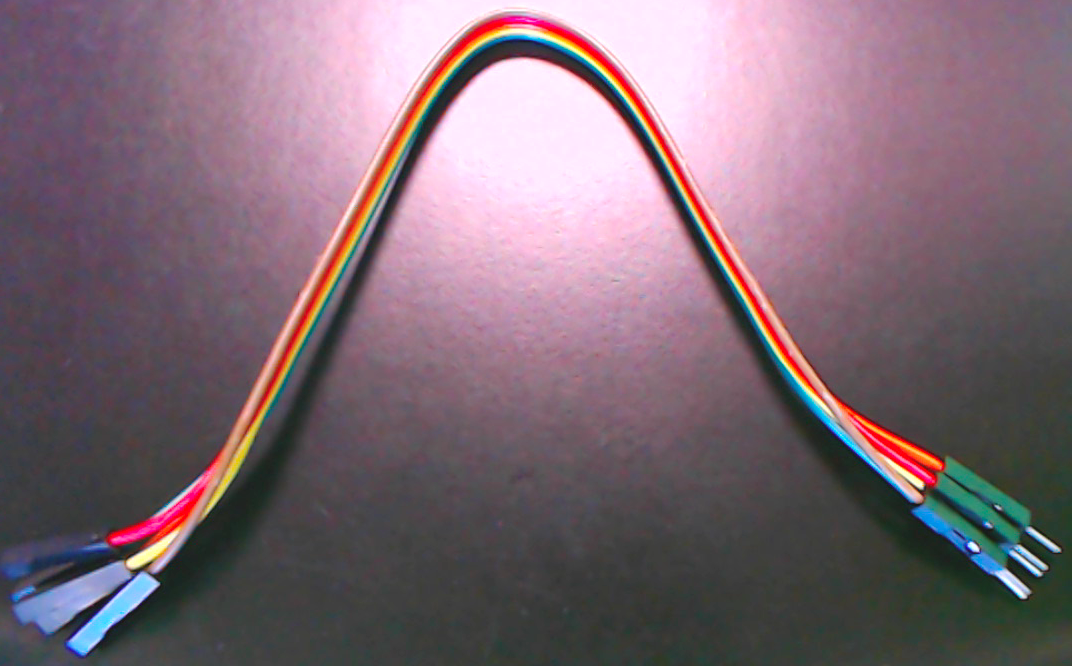
\includegraphics[height=2cm]{fm-5cable}}
}{}
\ifdefstring{\displaymodule}{MAX7219matrix}{
    \renewcommand{\displaymoduleitem}{\item One (1) $8 \times 8$ LED matrix display module \\ \textbf{\textit{Add LED matrix image here}}} %\includegraphics[height=2cm]{inventory/max7219matrix}}
}{}
%! suppress = MissingImport
\ifdefstring{\displaymodule}{LCD1602}{
    \renewcommand{\displaymoduleitem}{
        \item One (1) $2 \times 16$ character LCD display module \\ 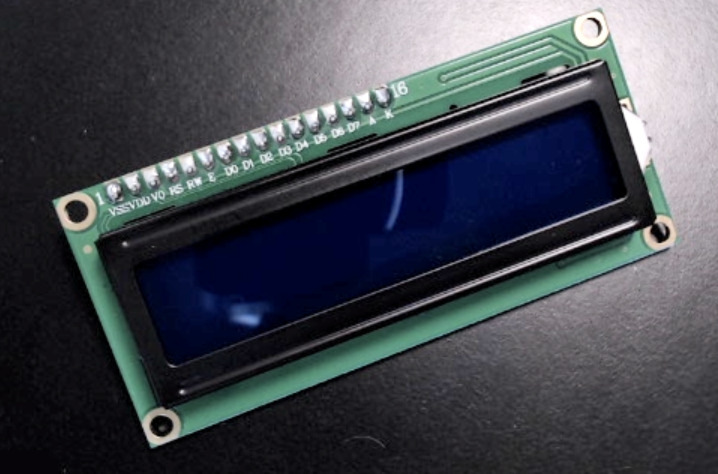
\includegraphics[height=2cm]{inventory/lcd1602}
        \ifdefstring{\serialprotocol}{I2C}{ \item One (1) I2C-LCD Serial Interface (might be attached to display module) \\ 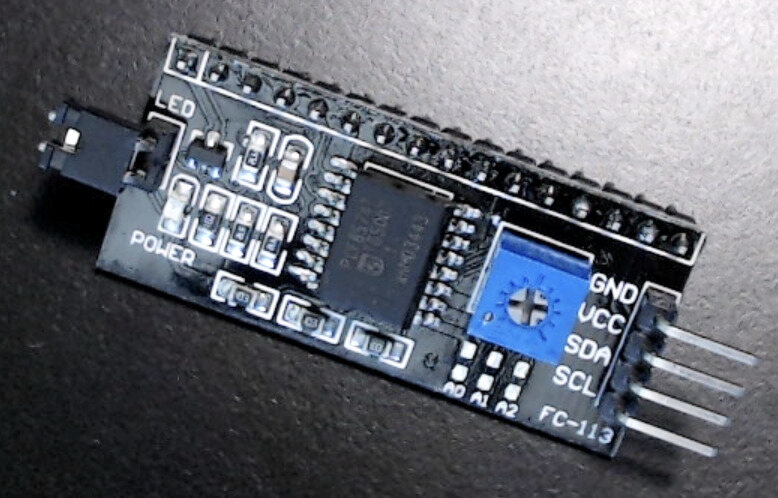
\includegraphics[height=2cm]{inventory/lcd-adapter} \hspace{1cm} or \hspace{1cm} 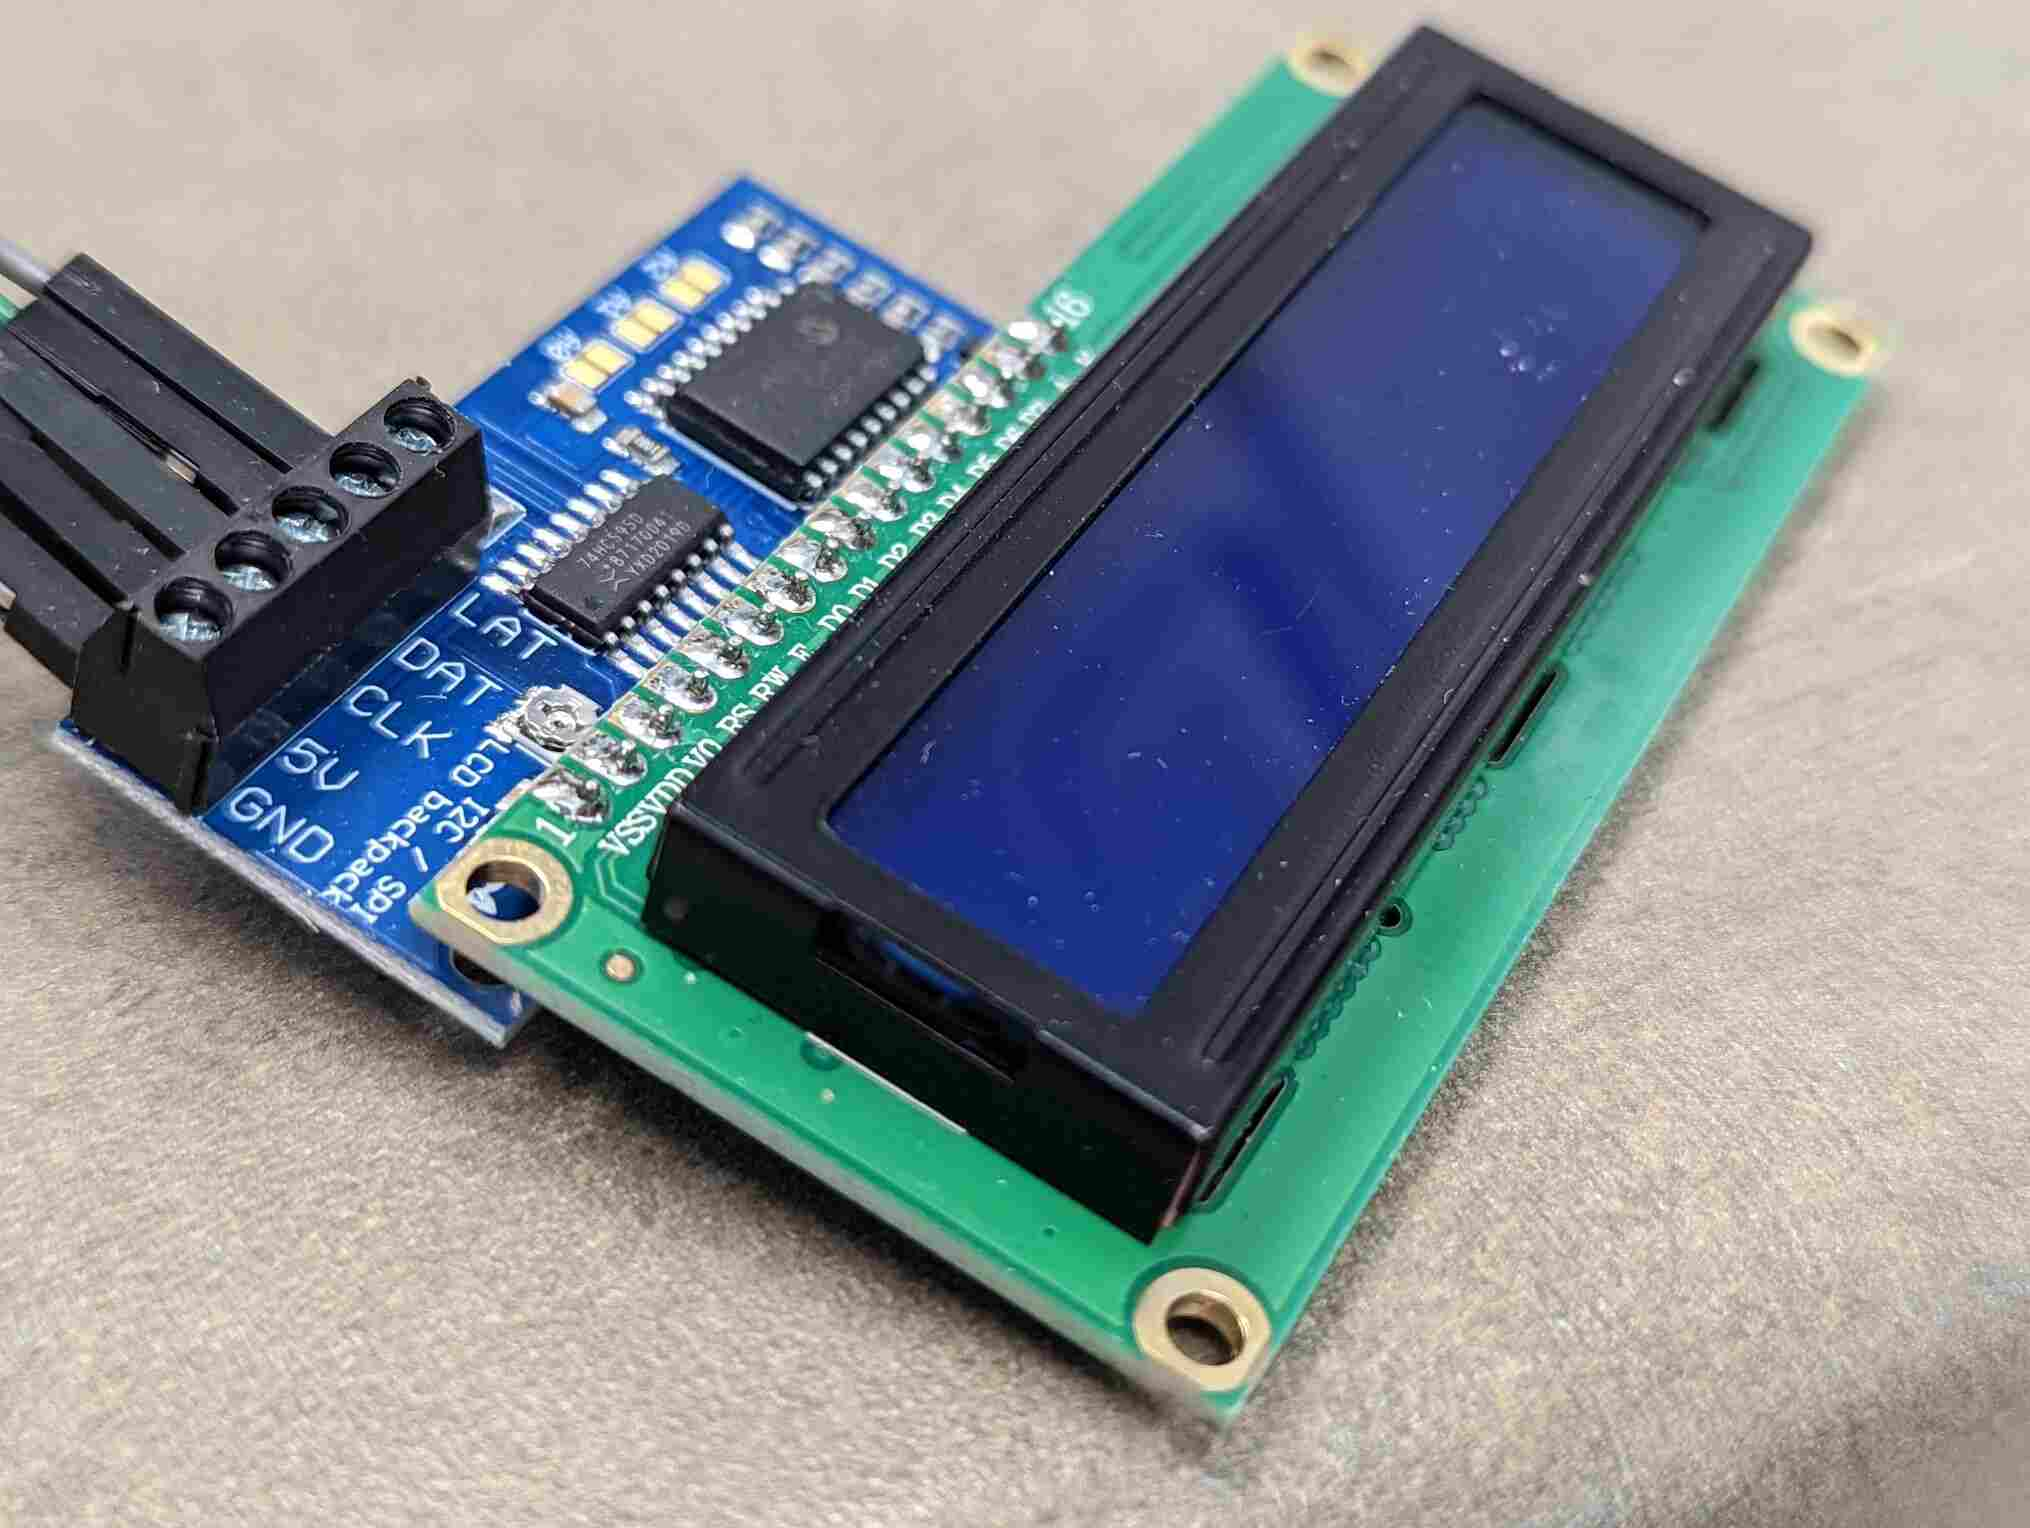
\includegraphics[height=2cm]{inventory/adafruit-lcd-adapter} \hspace{1cm} or \hspace{1cm} 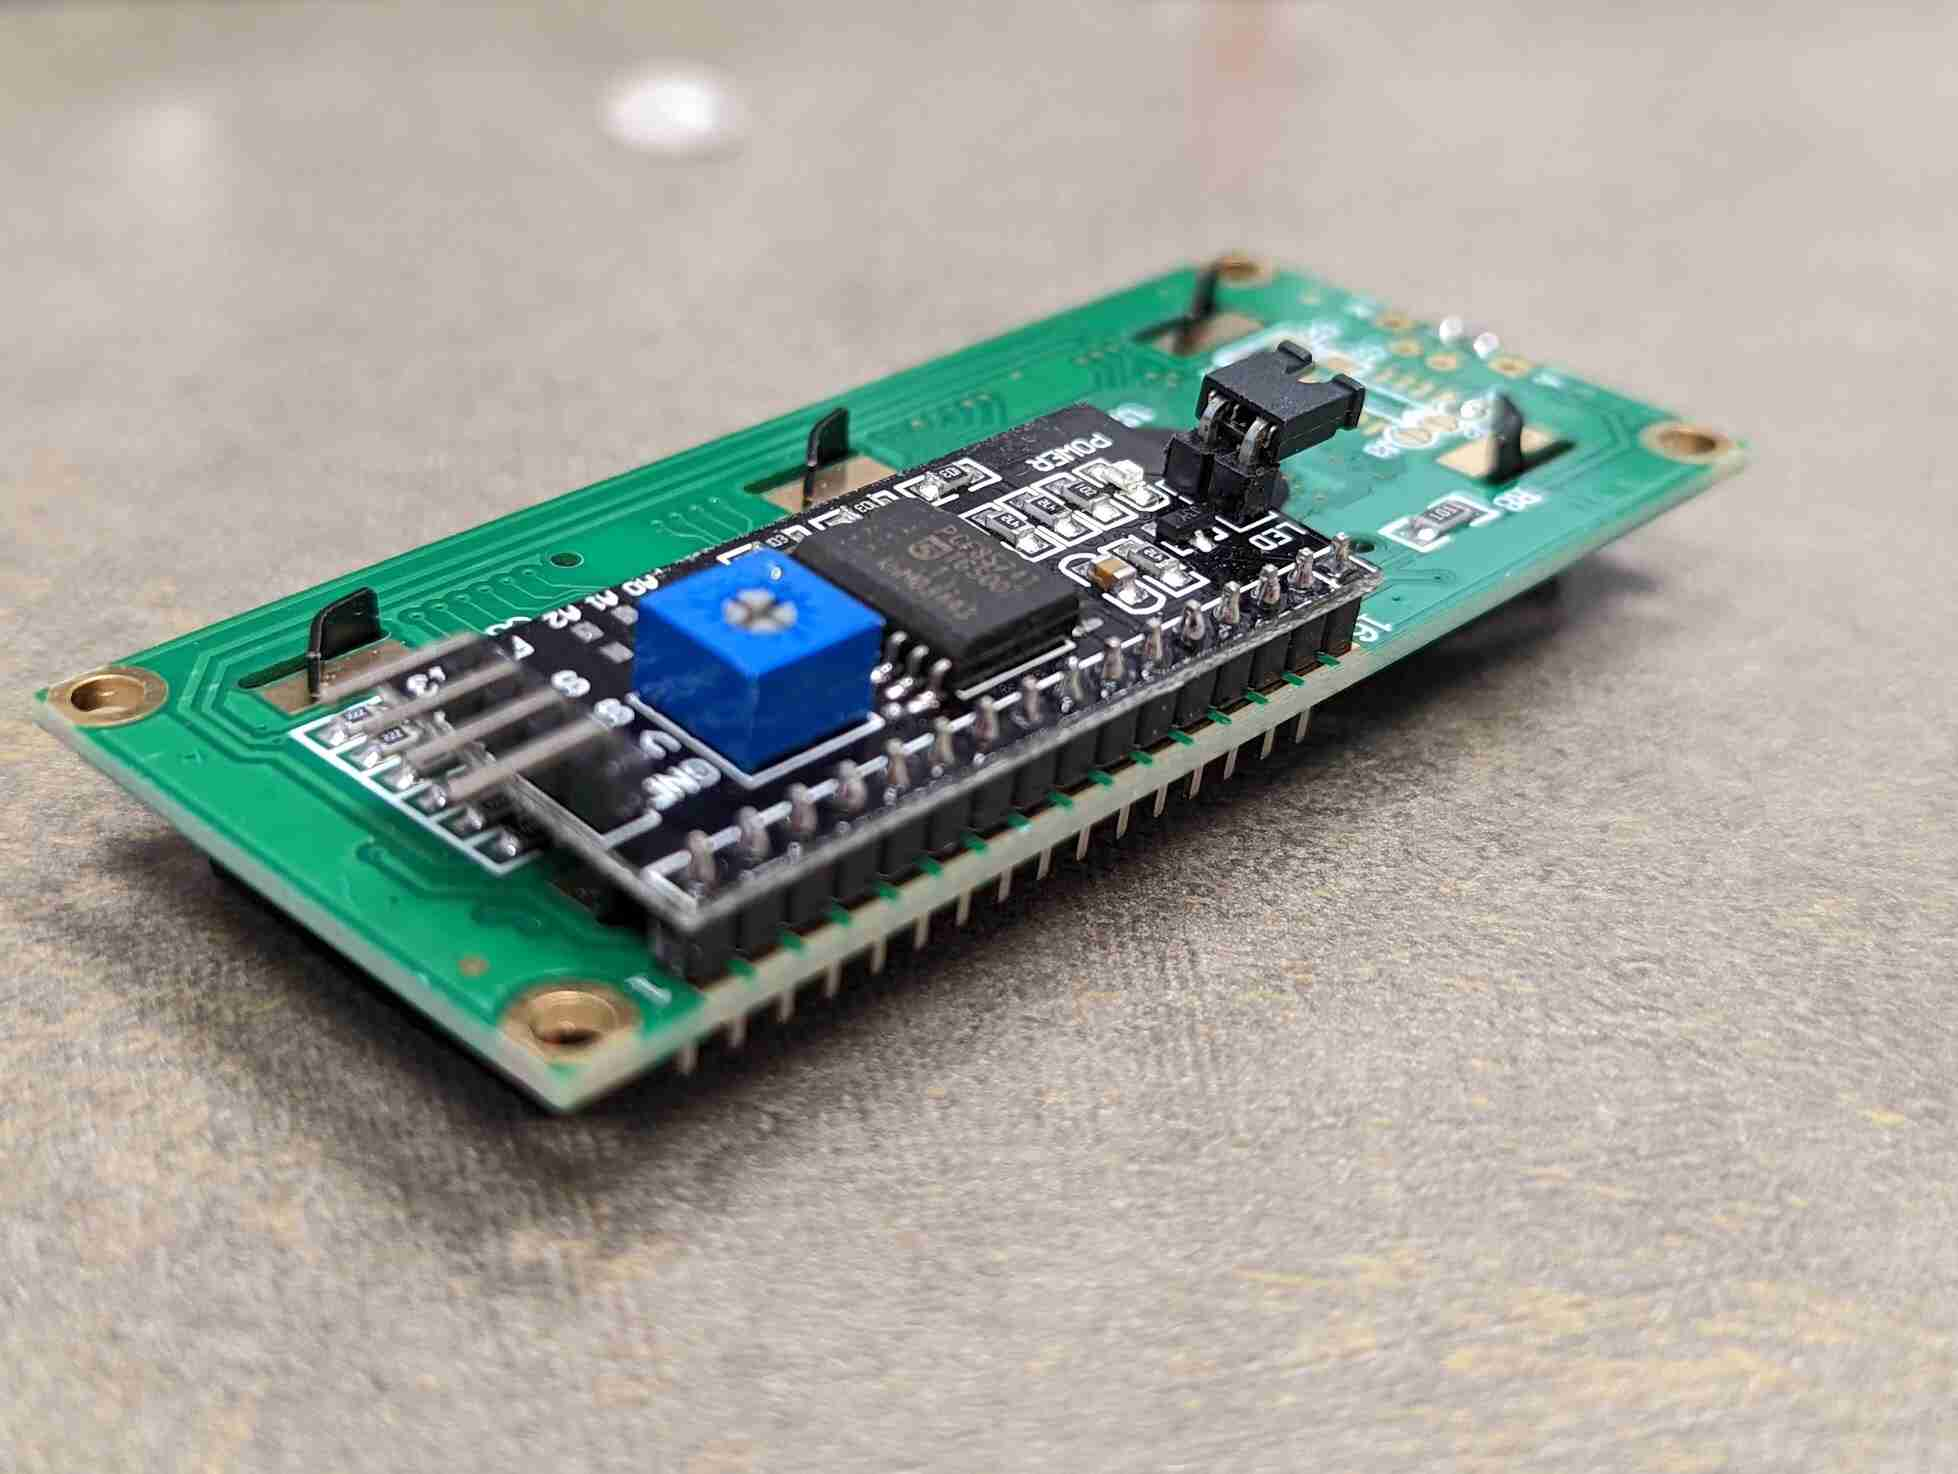
\includegraphics[height=2cm]{inventory/piggyback-lcd-adapter} }{}
        \ifdefstring{\serialprotocol}{SPI}{\item One (1) 74HC595 8-bit shift register \\ \textbf{\textit{Add shift register image here}}}{} %\includegraphics[height=2cm]{inventory/shiftregister}}{}
    }
    \ifdefstring{\serialprotocol}{I2C}{\renewcommand{\fmcableitem}{\item One (1) 4-conductor 20cm ``rainbow'' cable (female-to-male) \\ 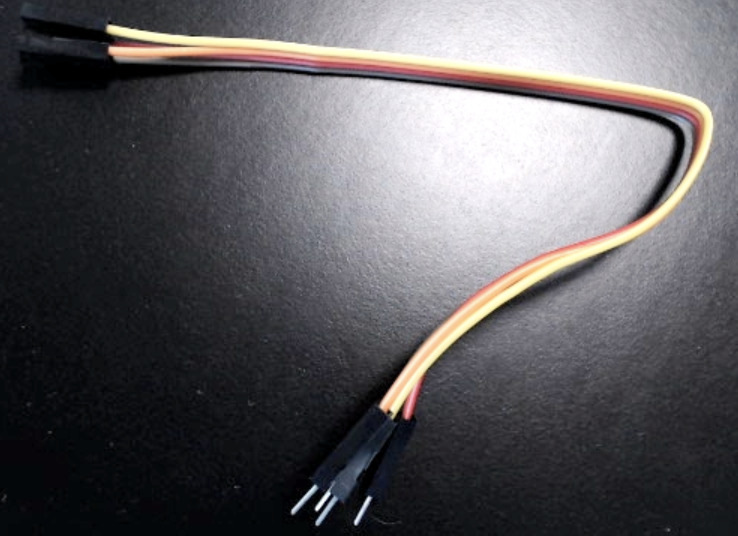
\includegraphics[height=2cm]{inventory/fm-4cable}}}{}
}{}

%%%%%%%%%%

Examine the contents of your class kit.
It contains:

%! suppress = MissingImport
\begin{itemize}
    \item One (1) full-sized solderless breadboard \\
        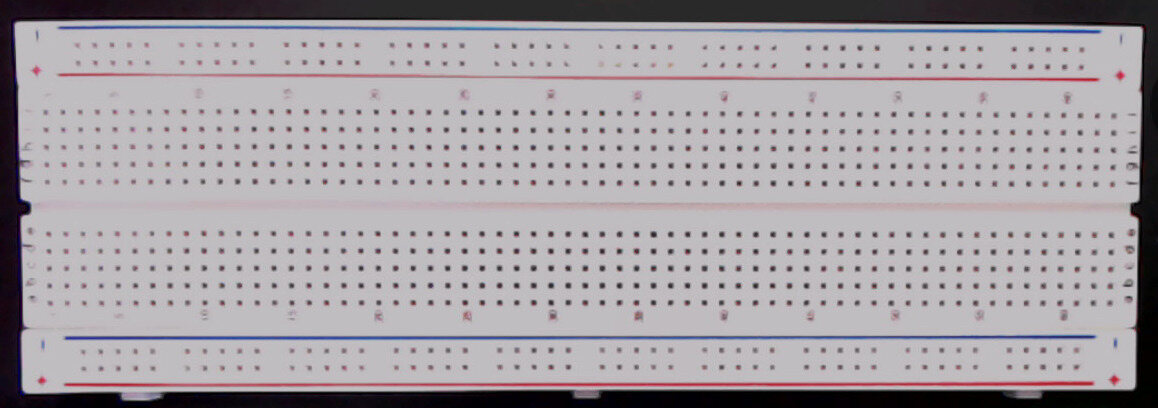
\includegraphics[height=2cm]{inventory/breadboard}
    \item One (1) \developmentboard\ (or clone) microcontroller board \\
        \devboardimage
    \item One (1) USB cable (mini-USB shown;
        yours may be different) \\
        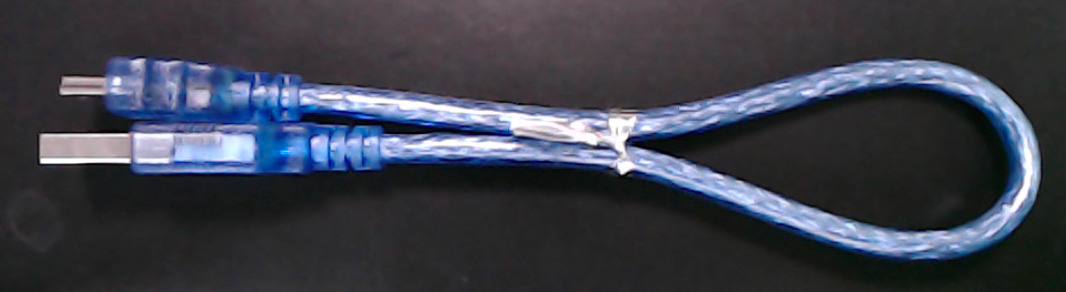
\includegraphics[height=2cm]{inventory/usb}
    \nandchipitem
    \item One (1) $4 \times 4$ matrix keypad \\
        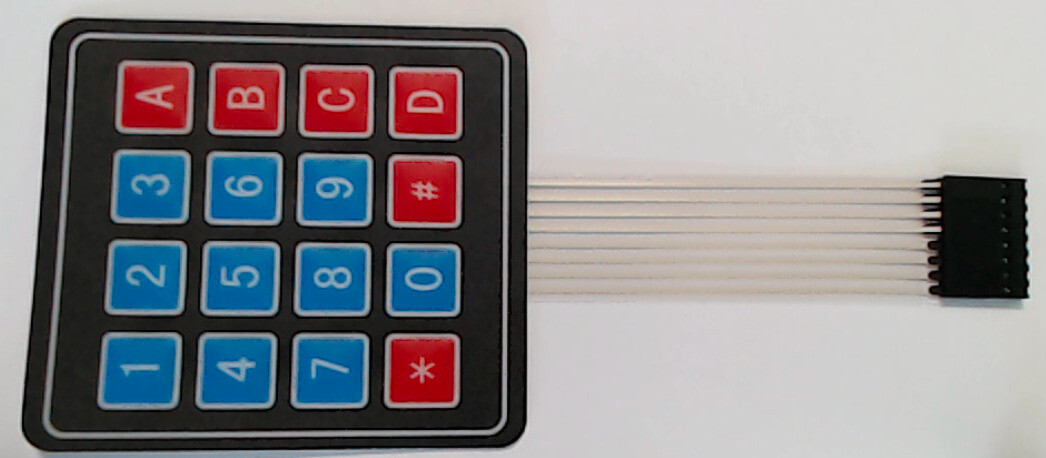
\includegraphics[height=2cm]{inventory/keypad}
    \item One (1) 8-pin male-male header strip (might already be inserted into keypad's female connectors;
        might have more than 8 pins) \\
        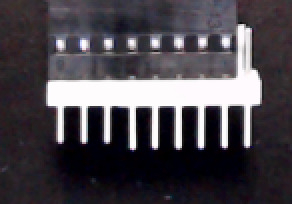
\includegraphics[height=2cm]{inventory/keypad-header-in-connector} \hspace{1cm} or
        \hspace{1cm} 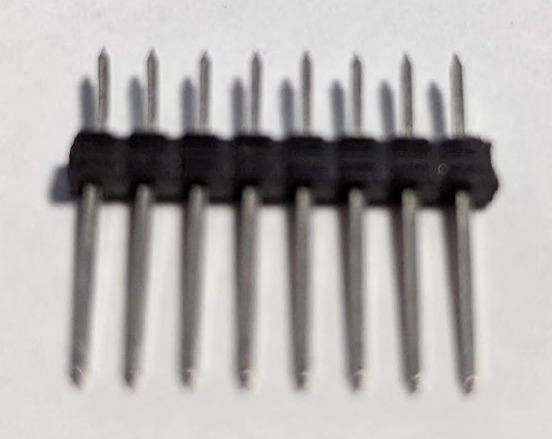
\includegraphics[height=2cm]{inventory/keypad-header-without-connector}
    \item Two (2) breadboard-mount momentary pushbuttons, aka tactile switches;
        these might have two leads (which might or might not be attached to cardboard strip), or they might have 4 prongs \\
        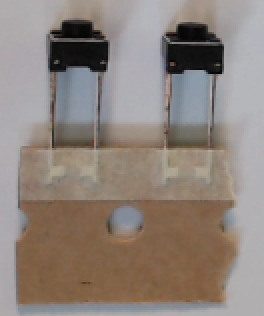
\includegraphics[height=2cm]{inventory/buttons-2pin} \hspace{1cm} or
        \hspace{1cm} \textbf{\textit{Add 4-prong image here}} %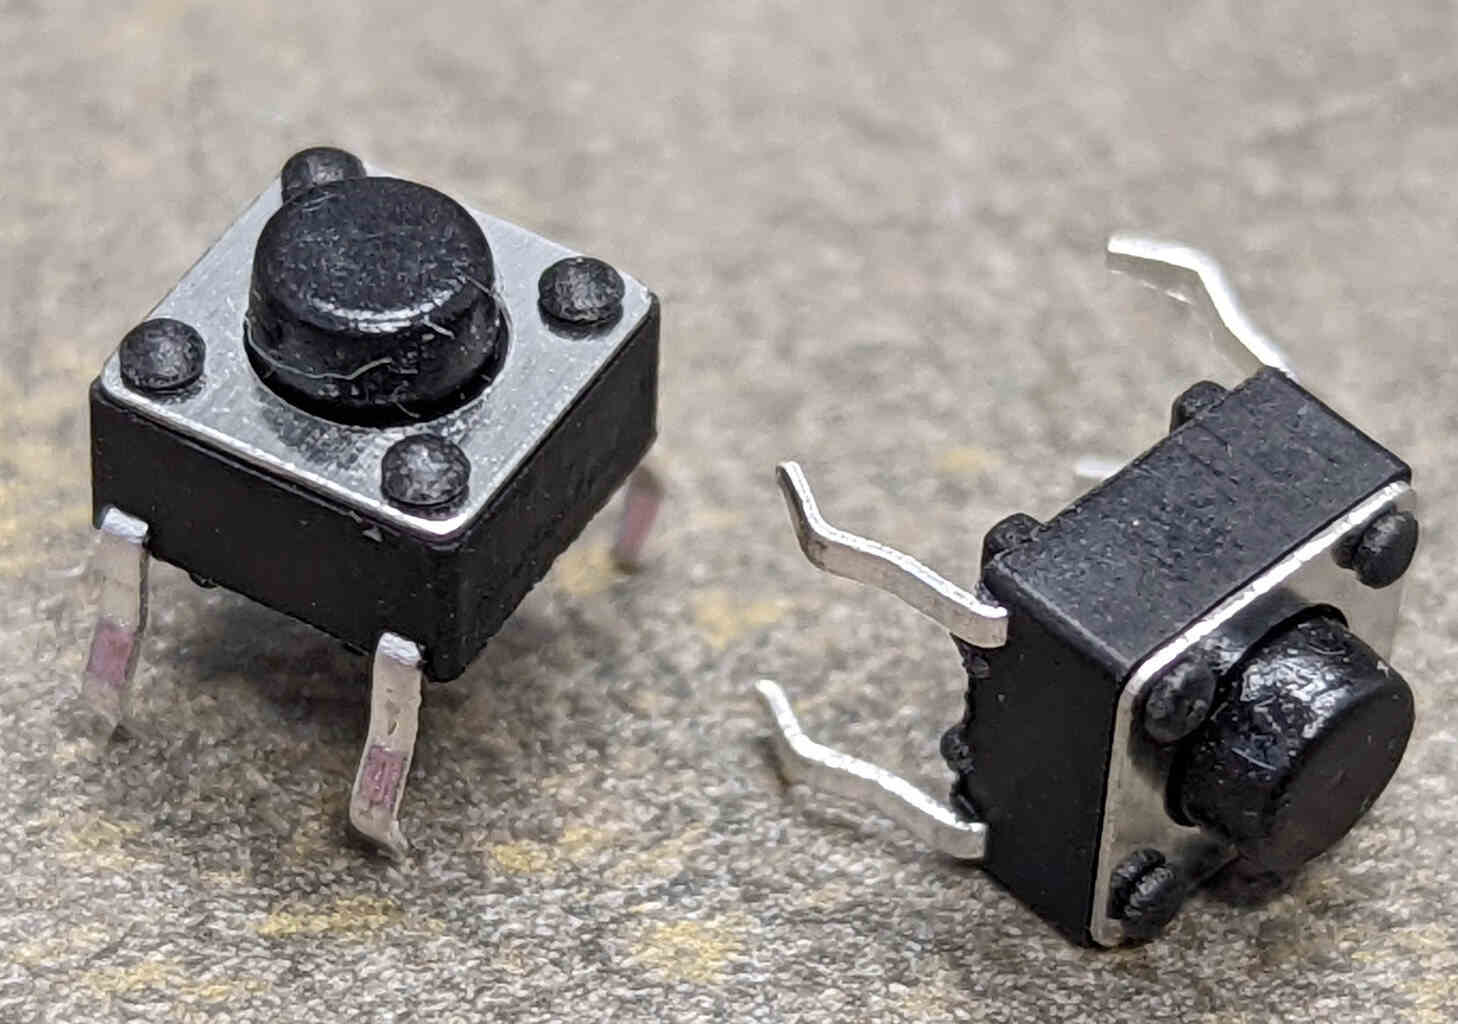
\includegraphics[height=2cm]{inventory/buttons-4pin}
    \item Two (2) breadboard-mount slide switches;
        these might have three pins spaced 0.1in (2.54mm) apart, or they might have two pins spaced 0.3in (7.62mm) apart. \\
        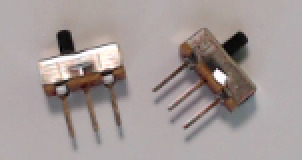
\includegraphics[height=2cm]{inventory/sliders-spdt} \hspace{1cm} or
        \hspace{1cm} \textbf{\textit{Add dip switch image here}} %\includegraphics[height=2cm]{inventory/sliders-dip1}
    \displaymoduleitem
    \item One (1) Light Emitting Diode (LED) (color may be different from shown) \\
        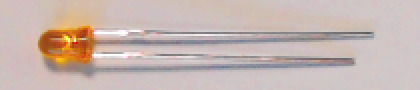
\includegraphics[height=1cm]{inventory/led}
    \item One (1) 1k$\Omega$ resistor \\
        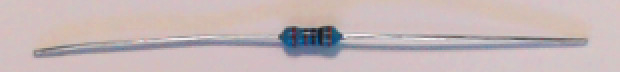
\includegraphics[height=1cm]{inventory/resistor}
    \item One (1) 40-conductor 10cm ``rainbow'' cable (male-to-male), \textit{or} One (1) 20-conductor 10cm ``rainbow'' cable (male-to-male) and one (1) 20-conductor 20cm ``rainbow'' cable (male-to-male) \\
        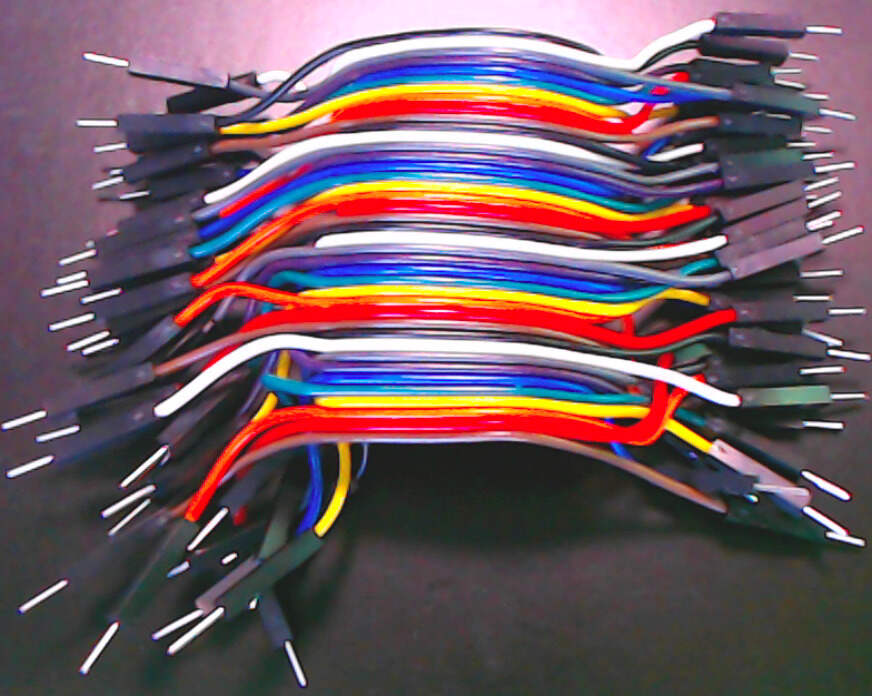
\includegraphics[height=2cm]{inventory/mm-cable}
    \fmcableitem
\end{itemize}

There may be other items in the class kit.
Set these aside;
you will not need them for this prelab, though they may be used in a specific lab.


\vspace{0.5cm}

\section*{Assembling the Class Kit}

    You will assemble the hardware in the following steps.
    \textbf{At various checkpoints, you should pause to have a TA or classmate double-check your work.}
    When you do so, update the \textit{checkpoints.txt} file to indicate who checked your work and when they did so.

    You may want to store your partially- and fully-completed kit in a plastic food container or some other container to prevent jumper wires from being pulled out while in your backpack.

    \textit{
        \textbf{Note 1:} The following pages include diagrams and some photographs of the assembly.
        The wire colors in the diagrams do not match the wire colors in the assembly.
        The wire colors in the diagrams are coded by the purpose they serve, whereas the wire colors in the photographs are the colors of wires removed from the \rainbow.
    }

    \textit{
        \textbf{Note 2:} The circuit you build by following these instructions will look a bit like a rat's nest (Figure~\ref{fig:complete-kit}) by the time that you are finished.
        This is because the jumper wires you remove from the \rainbow\ are not cut to length and generally will be longer than they need to be (which is much better than being shorter than they need to be).
        If you have prior experience with building circuits on a solderless breadboard, and if you have solid-core wires and wire cutters, then \underline{optionally} you may build the circuit with cut-to-length solid core wires.
    }

\section{Microcontroller and IDE}                           %! suppress = MissingImport
\newcommand{\microcontrollerreference}{}
\newcommand{\pindescription}{}
\newcommand{\icspdescription}{}
\newcommand{\usartdescription}{}
\newcommand{\digitalpindescription}{}
\newcommand{\analogpindescription}{}
\newcommand{\regulatedvoltagedescription}{}
\newcommand{\unregulatedvoltagedescription}{}
\newcommand{\resetdescription}{Finally, the \texttt{RESET} pins will reset the \developmentboard\ if grounded (pressing the button in the middle of the \developmentboard\ will also reset it).}
\newcommand{\microcontrollerprocessorandmemory}{}
\newcommand{\microcontrollerintegertiming}{}
\newcommand{\microcontrollerdivisionandfloats}{There is no hardware divider, and there is no floating point hardware, so integer division (to include the modulo operation) and all floating point operations are performed in software, requiring hundreds of clock cycles.}
\newcommand{\memorymodeldescription}{If you have already read the first half of Chapter 8, the \microcontroller\ has separate instruction and data memory, similar to the simple processor design described in the first half of Chapter 8.}
\newcommand{\pipelinedescription}{If you have already read the second half of Chapter 8, the \microcontroller\ has a 2-stage pipeline (with \textit{Fetch} and \textit{Execute} stages).}

%! suppress = NonMatchingIf
\ifdefstring{\microcontroller}{ATmega328P}{
    \renewcommand{\microcontrollerreference}{Atmel ATmega328P\footnote{\url{https://ww1.microchip.com/downloads/en/DeviceDoc/Atmel-7810-Automotive-Microcontrollers-ATmega328P_Datasheet.pdf}}}
    \renewcommand{\icspdescription}{The six upward-pointing pins are used to program the \developmentboard\ without using a host computer; we will not use these.}
    \renewcommand{\usartdescription}{\texttt{RX0} and \texttt{TX1} are used for asynchronous serial communication; as the USB interface also uses the same corresponding pins on the \microcontroller, we will not use these two pins (you will notice that when the \developmentboard\ communicates with the host computer, the \texttt{RX} and \texttt{TX} LEDs will illuminate).}
    \renewcommand{\microcontrollerprocessorandmemory}{an 8-bit processor with 32KB of flash memory for the program and 2KB of RAM for data}
    \renewcommand{\microcontrollerintegertiming}{While 8-bit logical operations, as well as 8-bit addition and subtraction, can be completed in one clock cycle, multiplication requires two clock cycles (16-bit operations require additional clock cycles).}
}{}

%! suppress = NonMatchingIf
\ifdefstring{\formfactor}{nano}{
    \renewcommand{\analogpindescription}{Pins \texttt{A0}-\texttt{A7} are analog input pins; however, \texttt{A0}-\texttt{A5} can also be used as digital input/output pins \texttt{D14}-\texttt{D19}. \texttt{AREF} (analog reference) is used to provide a reference voltage for the ADC (we will not use this pin).}
    \renewcommand{\pindescription}{It has thirty downward-pointing pins.}
    \renewcommand{\digitalpindescription}{Pins \texttt{D2}-\texttt{D13} are digital input/output pins.}
    \renewcommand{\unregulatedvoltagedescription}{\texttt{VIN} can be used to power the \developmentboard\ if connected to an unregulated power supply, such as a 9V battery; the \developmentboard's onboard voltage regulator will then provide regulated voltages needed.}
}{}

%! suppress = NonMatchingIf
\ifbool{fivevolt}{
    \renewcommand{\regulatedvoltagedescription}{Pins \texttt{3V3} and \texttt{5V} provide regulated 3.3 volts and 5 volts for external circuitry; \texttt{5V} can also be used to power the \developmentboard\ if connected to a regulated 5V power supply.}
}{
    \renewcommand{\regulatedvoltagedescription}{The \texttt{3V3} pin provides regulated 3.3 volts for external circuitry; it can also be used to power the \developmentboard\ if connected to a regulated 3.3V power supply. The \texttt{VUSB} pin can provide regulated 5 volts only if the \texttt{VUSB} jumper pads on the \developmentboard's underside are soldered together.}
}

%%%%%%%%%%

A microcontroller, such as the \microcontrollerreference\ on the \developmentboard, is a very simple processor when compared to a microprocessor designed for general-purpose computing.
At the same time, a microcontroller has some features not present on a microprocessor, such as built-in analog-to-digital converters (ADCs).\footnote{We will not use the ADCs in the I/O labs.} A microcontroller board, such as the \developmentboard, combines the microcontroller with other components\footnote{Typically, a voltage regulator, a crystal oscillator, and a USB interface.} in a form factor convenient for experimentation.

The \developmentboard\ has a USB port to connect to a computer and/or to provide power to the \developmentboard.
\icspdescription\
\pindescription\
\usartdescription\
\digitalpindescription\
\analogpindescription\
\regulatedvoltagedescription\
\unregulatedvoltagedescription\
The \texttt{GND} pins are for the common ground;
the ground portions of external circuitry and of external power supplies must be electrically connected to the \developmentboard's ground.
\resetdescription
Note that, unlike a general-purpose computer, when a microcontroller is reset it will restart its program when the reset is released.

The \microcontroller\ microcontroller on the \developmentboard\ is \microcontrollerprocessorandmemory.
\microcontrollerintegertiming\
\microcontrollerdivisionandfloats\

\memorymodeldescription\
\pipelinedescription\
If you have already read Chapter 10, the \microcontroller\ does not have cache memory;
however, the data memory is SRAM, the same memory technology used in microprocessors' memory caches.
If you have already read Chapter 10, the \microcontroller\ does not have a memory management unit for virtual memory;
instead, the \microcontroller\ uses only physical addressing.

\subsection{Breadboard Terminology}

    \begin{description}
        \checkoffitem{If you are not familiar with solderless breadboards, read the
        \href{https://learn.adafruit.com/breadboards-for-beginners?view=all}{Breadboards for Beginners} Guide at adafruit.com.}
    \end{description}

    Even though breadboards are often viewed in ``landscape'' orientation (such as in the photo in Section~\ref{sec:inventory} and as seen in the diagram figures) instead of ``portrait'' orientation, the numbered sections are called rows and the lettered sections are called columns.
    In the interest of preserving common usage, we will use this terminology.
    We will refer to specific contact points using the letter-number combination.

\subsection{Optional: Breadboard Templates}                    %! suppress = MissingImport
Figure~\ref{fig:templates} is a set of two %four
templates for the Cow Pi circuit %(one for each combination of pushbuttons (2-lead or 4-prong) and slide-switches (2-pin or 3-pin).
(one with 2-lead pushbuttons and one with 4-prong pushbuttons)
Each dot (\tikz{\draw[white,fill=gray] (0,0) +(0,3pt) circle (1pt);}) represents a breadboard contact point.
Each dot with a circle (\tikz{\drawtarget{0}{3pt} \draw[white,fill=gray] (0,0) +(0,3pt) circle (1pt);}) is a contact point in which you will insert a jumper lead.
Attached to most of these circles is the contact point for the other end of the jumper wire (\tikz{\drawlabelledtarget{0}{0}{1}{k64} \draw[white,fill=gray] (0,0) circle (1pt);}).
The font for these labels is unfortunately small;
there is no avoiding this problem
(you can use a magnifying glass or your mobile phone's camera on magnification if you have difficulty reading the labels).
The footprints of several components are shown as light-gray outlines;
resistors (\tikz{\ctikzset{bipoles/resistor/height=0.2}\ctikzset{bipoles/resistor/width=0.3}\draw (0,0) to[R] (1,0)}) and LEDs (\tikz{\ctikzset{bipoles/diode/height=0.2}\ctikzset{bipoles/diode/width=0.2}\draw (0,0) to[led] (1,0)}) are shown using their conventional symbols.
Squares (\tikz{\draw[white,fill=gray] (0,0) +(2pt,3pt) circle (1pt); \draw (0,0) +(0,1pt) rectangle +(4pt,5pt);}) are where you'll insert component individual pins,
and rectangles (\tikz{\draw (0,0) +(0,1pt) rectangle +(11pt,5pt); \draw[white,fill=gray] (0,0) +(2pt,3pt) circle (1pt); \draw[white,fill=gray] (0,0) +(5.5pt,3pt) circle (1pt); \draw[white,fill=gray] (0,0) +(9pt,3pt) circle (1pt);}) are where you'll insert components' in-line pins.
Finally, the four corners (\tikz{\draw[white,fill=gray] (0,0) +(2pt,3pt) circle (1pt); \draw (0,1pt) -- (4pt,5pt); \draw (0,5pt) -- (4pt,1pt);}) are used to align the template on your solderless breadboard.

%TODO: add dip1 switch subfigures
\begin{figure}[p]
    \subfloat[Template that uses 3-pin slide-switches and 2-lead pushbuttons.]{
        \hspace{-.5in}
        \begin{tikzpicture}[x=.1in, y=.1in]
            \drawbreadboard
            \drawnano{1}{3}{Arduino Nano}
            \drawledcircuit
            \drawnand{18}{5}
            \drawswitches{\controlsstartat+1}
            \drawbuttons{\controlsstartat+11}{2}
            \drawkeypadandtargets{\controlsstartat}
            \drawdisplay{48}
        \end{tikzpicture}
    }
    \vspace{.5in}
    \subfloat[Template that uses 3-pin slide-switches 4-prong pushbuttons.]{
        \hspace{-.5in}
        \begin{tikzpicture}[x=.1in, y=.1in]
            \drawbreadboard
            \drawnano{\mcux}{\mcuy}{Arduino Nano}
            \drawledcircuit
            \drawnand{\nandx}{\nandy}
            \drawswitches{\controlsstartat+1}
            \drawbuttons{\controlsstartat+11}{4}
            \drawkeypadandtargets{\controlsstartat}
            \drawdisplay{48}
        \end{tikzpicture}
    }
    \caption{Templates to improve accuracy when constructing the Cow Pi circuit on a solderless breadboard.}\label{fig:templates}%\addcontentsline{toc}{section}{Breadboard Templates}
\end{figure}

\underline{\textbf{\textit{Optionally}}:}
\begin{description}
    \checkoffitem{Print the page that has the template appropriate to your particular switches and pushbuttons.}
        \begin{itemize}
            \item When (if) you do so, be sure to select ``Actual size'' (see Figure~\ref{fig:printmenu}).
            If you mistakenly select a different option, the template will not line up properly with your breadboard: even a tiny scaling factor will add-up over the length of the breadboard.
        \end{itemize}
    \checkoffitem{Using the lead from a jumper wire, punch holes into the four $\times$s at the corners (contact points a1, j1, a63, and j63); see Figure~\ref{fig:punchingholes}.}
    \checkoffitem{Place the lead from a jumper wire into each of the four holes, and insert the leads into the corresponding contact points on the breadboard, pinning the template to the breadboard.}
    \checkoffitem{Confirm that the four jumpers are aligning the template to the breadboard by visually checking that the four leads are in the breadboard's contact points a1, j1, a63, and j63 (see Figure~\ref{fig:confirmalignment}).}
\end{description}

\begin{figure}
    \centering
    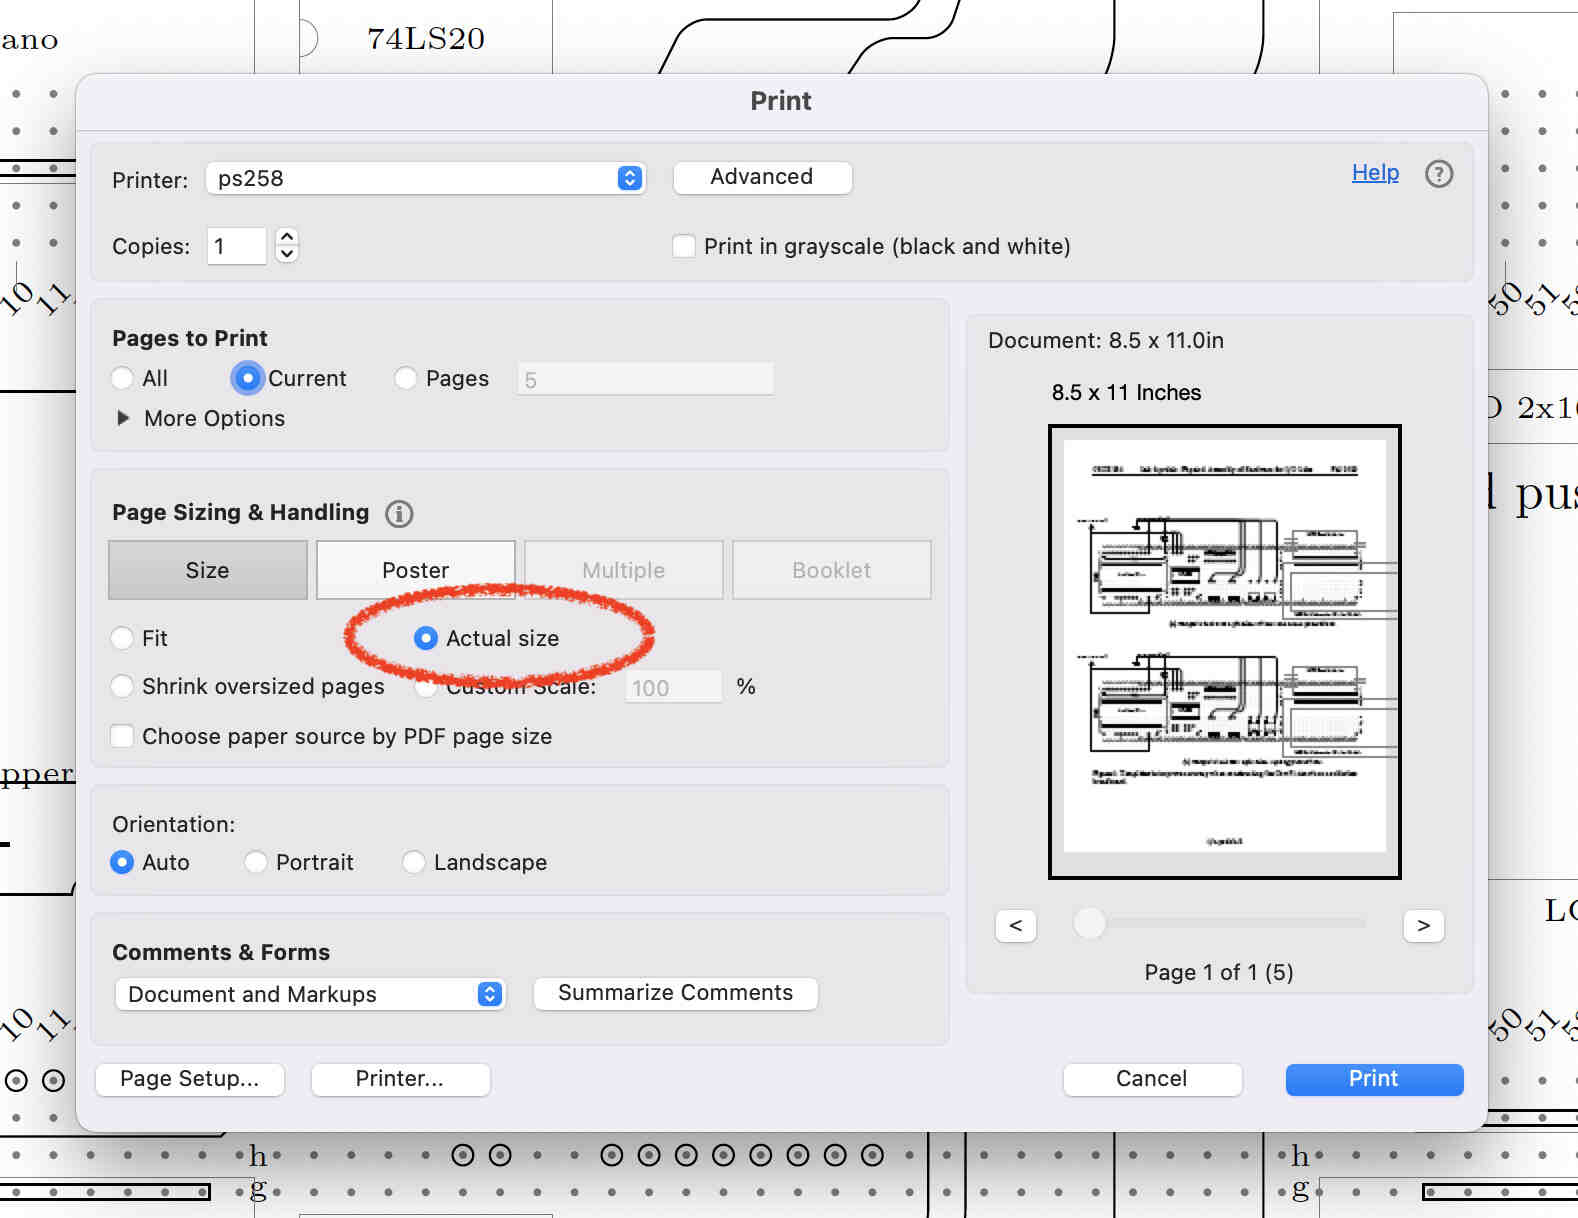
\includegraphics[width=0.5\textwidth]{breadboard-guides/print-menu}
    \caption{When printing a breadboard template, be sure to select ``Actual size''.} \label{fig:printmenu}
\end{figure}

\begin{figure}
    \centering
    \subfloat[Punching alignment holes in breadboard template.]{
        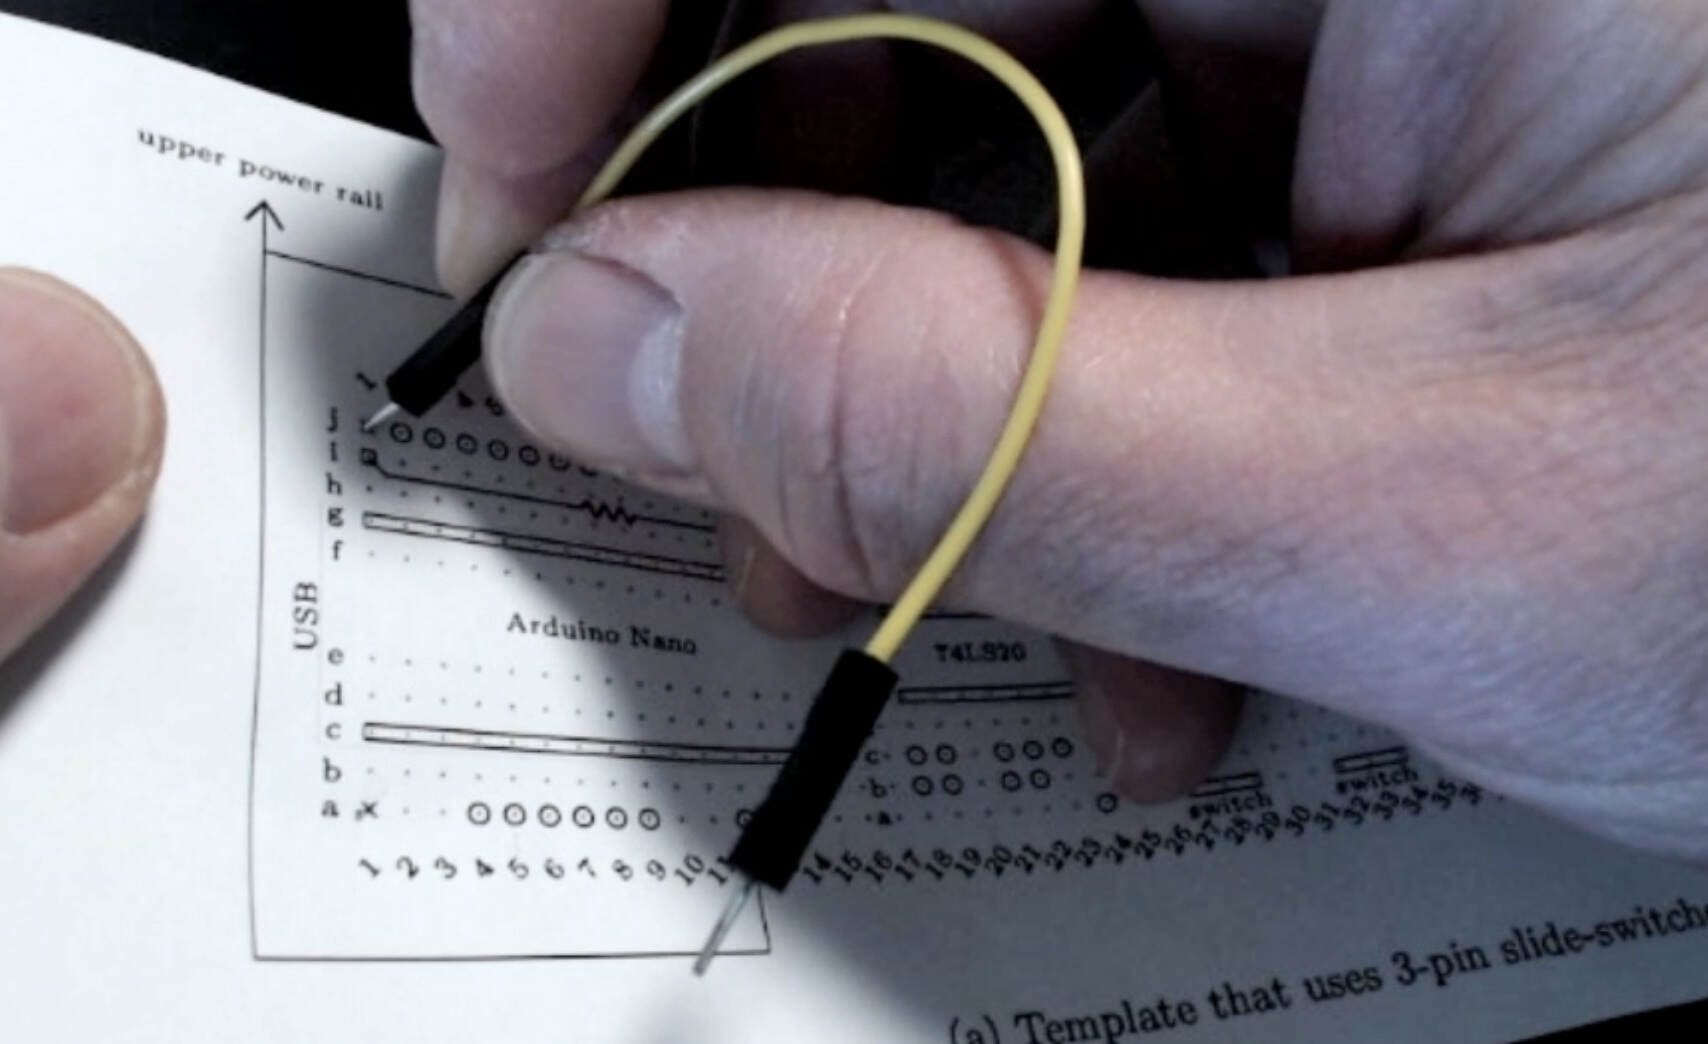
\includegraphics[height=3cm]{breadboard-guides/punching-holes}
        \label{fig:punchingholes}
    }
    \hfil
    \subfloat[Confirming that the corners of the template are aligned with the corners of the breadboard.]{
        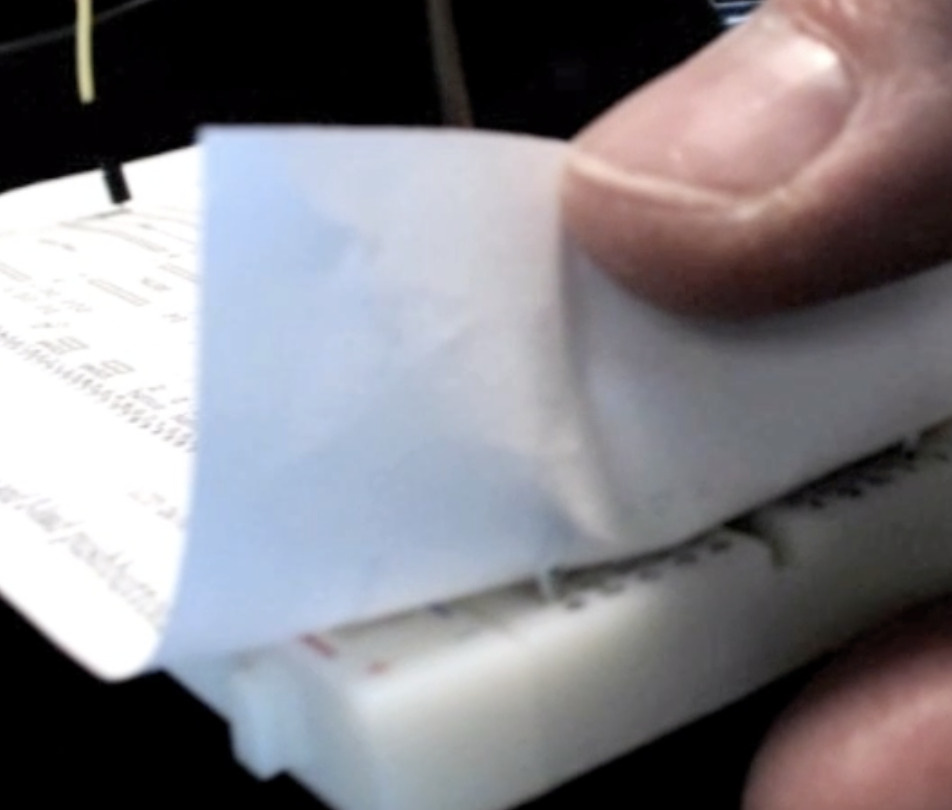
\includegraphics[height=3cm]{breadboard-guides/confirm-alignment}
        \label{fig:confirmalignment}
    }
    \caption{Preparing a breadboard template.}
\end{figure}



%! suppress = MissingImport
\subsection{Install the \developmentboard\ onto the Breadboard}

    \begin{description}
        \checkoffitem{Orient the breadboard in front of you so that row 1 is on your left and row 63 is on your right;
        column a should be at the bottom, and column j should be at the top.}
        \checkoffitem{\prepunch{\mcuupperrow\ and \mculowerrow}
        See Figure~\ref{fig:prepunching}.}
    \end{description}

    After the paper provides some initial resistance, the jumper's lead will slide into the breadboard's contact point;
    remove the lead and move on to the next contact point.
    You want to pre-punch these holes because the paper provides less resistance when you're inserting a single lead than it does when you're inserting a component with multiple leads.

    \begin{figure}
        \centering
        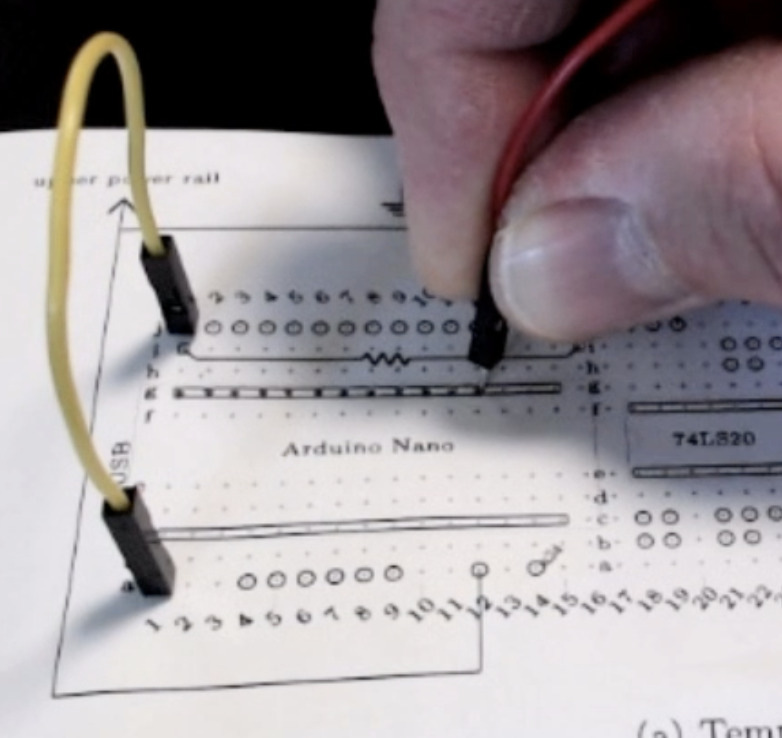
\includegraphics[height=3cm]{microcontroller/breadboard/prepunching}
        \caption{Pre-punching holes in the breadboard template before inserting a component.} \label{fig:prepunching}
    \end{figure}

    \begin{description}
        \checkoffitem{Remove the anti-static foam from the \developmentboard's pins.}
    \end{description}
    You will place the \developmentboard\ on the left side of the breadboard with the USB connector on the left (that is, facing away from the breadboard).
    \begin{description}
        \checkoffitem{Position the upper row of pins on contact points \mcuupperrow\ and the lower row of pins on contact points \mculowerrow.}
    \end{description}
%! suppress = NonMatchingIf
\ifdefstring{\formfactor}{nano}{
    The left side of the \developmentboard\ will obscure the labels for columns c--g.
    The right side of the \developmentboard\ will cover contact points c16--g16 but won't use them.
}{}
\begin{description}
    \checkoffitem{Double-check that:}  % TODO: figure out how to generalize this
        \begin{itemize}
            \item the pin labeled \texttt{D12} is in the upper-left, on contact point g1
            \item the pin labeled \texttt{D13} is in the lower-left, on contact point c1
            \item the pin labeled \texttt{VIN} is in the lower-right, on contact point c15
            \item the pin labeled \texttt{TX1} is in the upper-right, on contact point g15
        \end{itemize}
    \checkoffitem{Gently press on both ends of the \developmentboard\ to insert the pins into the contact points, using a slight rocking motion if necessary (Figure~\ref{fig:inserting-mcu}).}
    \checkoffitem{Press the \developmentboard\ into the breadboard until it physically cannot be inserted any deeper (Figure~\ref{fig:mcu-inserted}).}
\end{description}

%! suppress = NonMatchingIf
\begin{figure}
    \centering
    \subfloat[Press gently on both ends of the \developmentboard.] {
        \ifdefstring{\developmentboard}{Arduino Nano}{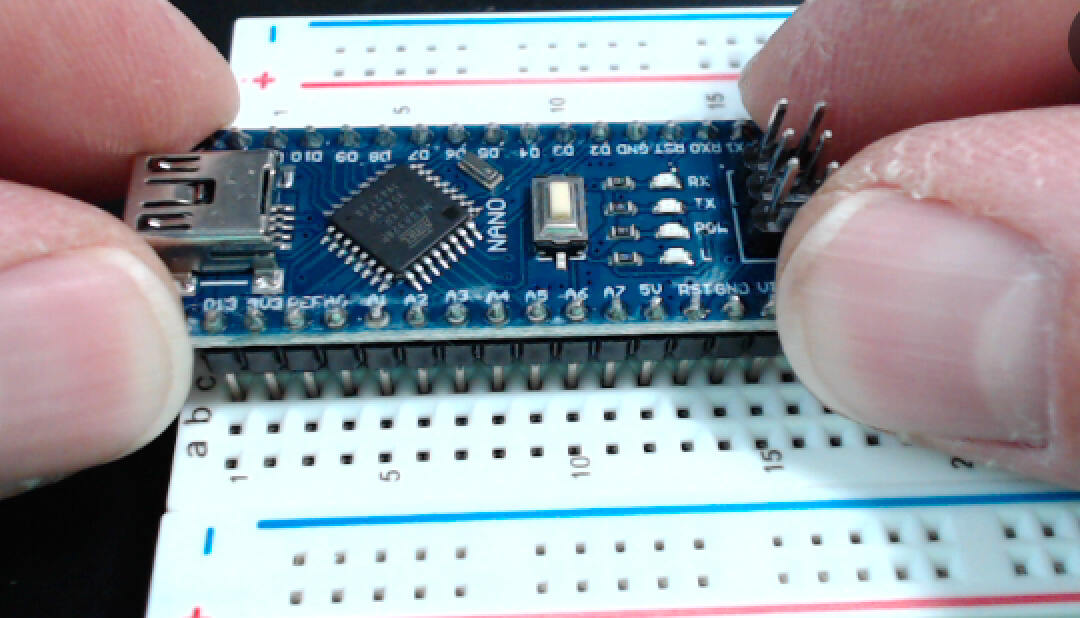
\includegraphics[height=3cm]{microcontroller/breadboard/inserting-nano}}{}
        \label{fig:inserting-mcu}
    }
    \hfil
    \subfloat[The \developmentboard\ fully inserted.] {
        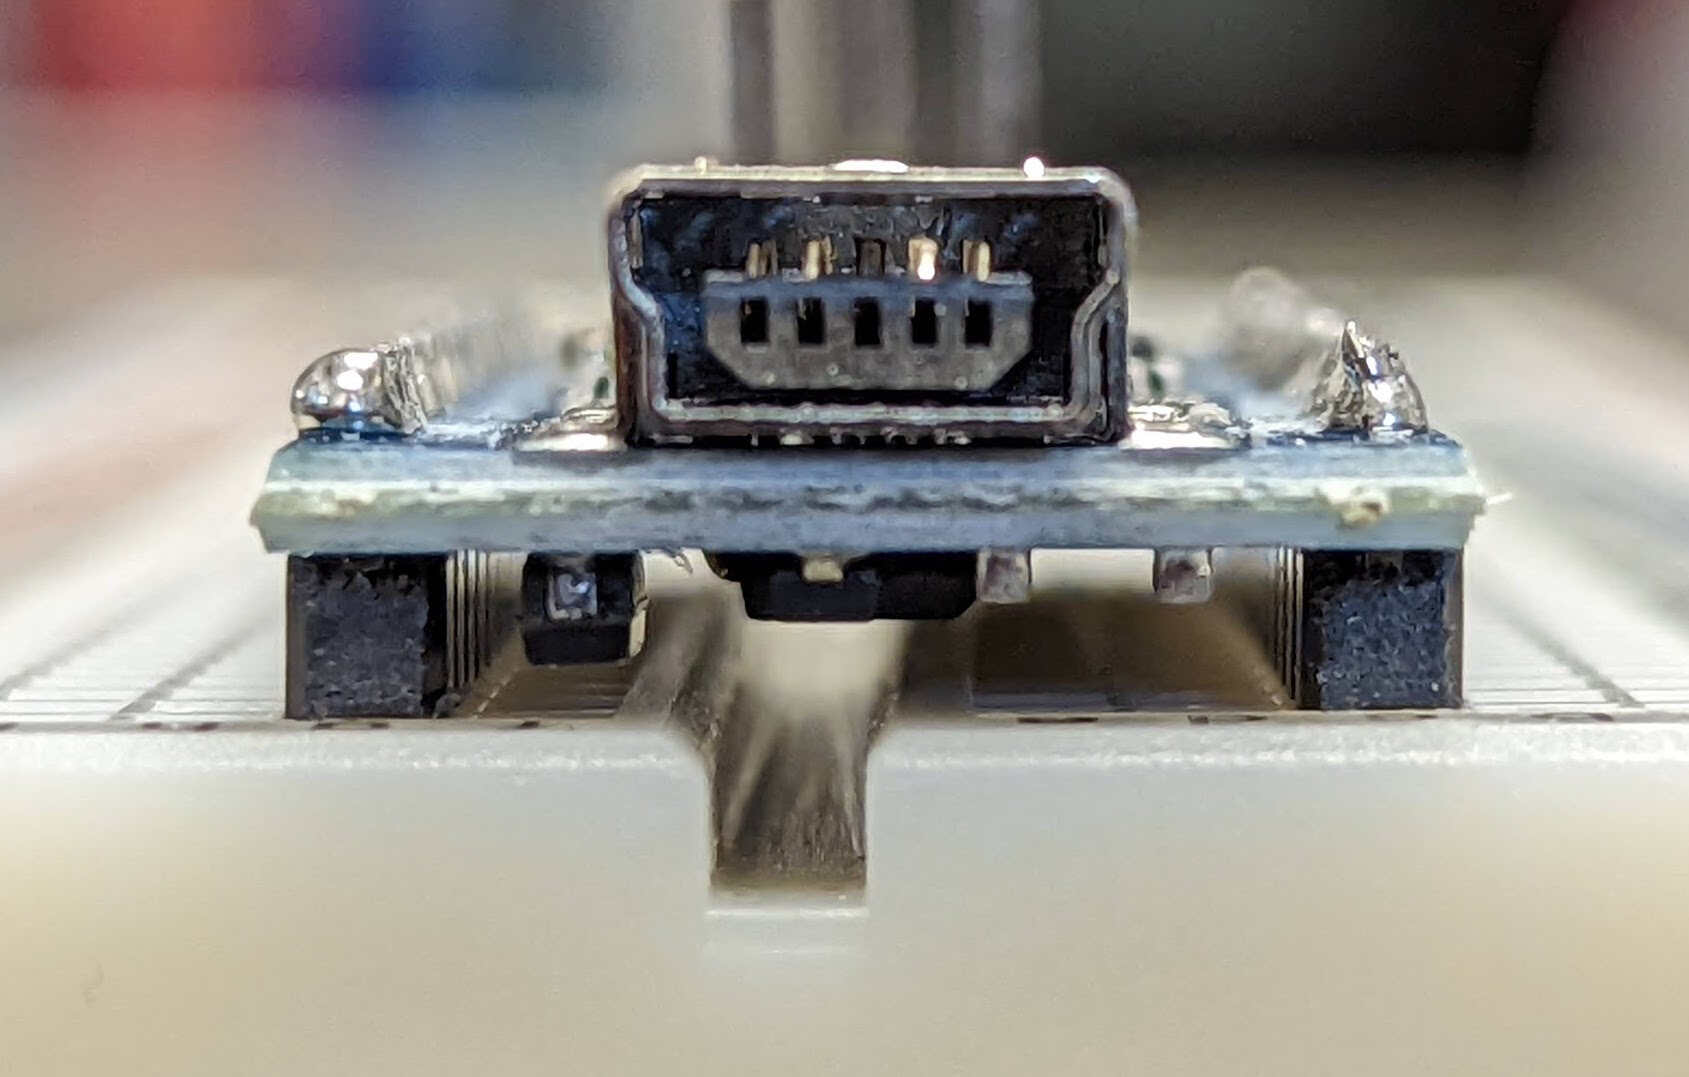
\includegraphics[height=3cm]{microcontroller/breadboard/nano-fully-inserted}
        \label{fig:mcu-inserted}
    }
    \caption{Inserting the \developmentboard\ into the breadboard.}
\end{figure}

\checkpoint{inserted the \developmentboard\ into the breadboard}

\textit{If you are using a breadboard template} then you can now remove the jumper wires from contact points a1 and j1;
the \developmentboard\ will keep the left side of the template pinned in place.


\subsection{Install Arduino IDE}

    The Arduino IDE is installed on the lab computers.
    If you choose to install the Arduino IDE on your personal laptop, you can download it from
    \url{https://www.arduino.cc/en/software}.
    Alternatively, you can install a browser plugin to use the
    \href{https://create.arduino.cc/projecthub/Arduino_Genuino/getting-started-with-arduino-web-editor-on-various-platforms-4b3e4a}{Arduino Web Editor}.
    There are third-party plugins for many other IDEs; however, using these may limit our ability to help you if your have difficulties.

\subsubsection*{About Arduino Programs}

    An Arduino program is called a \textit{sketch} for historical reasons.\footnote{The Arduino language is based off of the Wiring language, which in turn is based off of the Processing language, which was designed to make computing accessible to artists.}
    For all intents and purposes, you can think of it as a C++ program\footnote{Your code in the I/O labs will be C code.} in which you write two functions, \function{setup} and \function{loop}, along with any helper code that you need.
    The file extension for sketches is \textbf{\textit{.ino}} (as in, Ardu\textbf{\textit{ino}}).
    The Arduino IDE will compile your sketch and link it to a \function{main} function that looks something like:
    \begin{lstlisting}
    int main() {
        setup();
        while(true) {
            loop();
        }
    }
    \end{lstlisting}
    (The actual \function{main} function\footnote{\url{https://github.com/arduino/ArduinoCore-avr/blob/master/cores/arduino/main.cpp}} also calls a few other functions from the Arduino core library.)

\subsection{Connect to the \developmentboard}

    \begin{itemize}
        \item Connect one end of the mini-USB cable to a lab computer or to your personal laptop.\footnote{You can connect it to a ``wall wart'' USB power supply to run the \developmentboard, but you need to connect it to a computer to upload a new sketch to the \developmentboard.}
        \item Connect the mini-USB end of the cable to your \developmentboard.
    \end{itemize}
    The \texttt{PWR} LED will light up, and you may see the \texttt{L} LED repeatedly blink on-and-off.
    The \texttt{L} LED is connected to the \developmentboard's pin D13, and Arduino microcontroller boards typically leave the factory with \textit{Blink.ino} loaded, but it does not matter if yours does not have \textit{Blink.ino} pre-loaded.

    \begin{lstlisting}[basicstyle=\ttfamily\footnotesize]
    // the setup function runs once when you press reset or power the board
    void setup() {
      // initialize digital pin LED_BUILTIN as an output.
      pinMode(LED_BUILTIN, OUTPUT);
    }

    // the loop function runs over and over again forever
    void loop() {
      digitalWrite(LED_BUILTIN, HIGH);   // turn the LED on (HIGH is the voltage level)
      delay(1000);                       // wait for a second
      digitalWrite(LED_BUILTIN, LOW);    // turn the LED off by making the voltage LOW
      delay(1000);                       // wait for a second
    }
    \end{lstlisting}

    \begin{description}
        \checkoffitem{Open the Arduino IDE on the computer that your \developmentboard\ is connected to.}
        \checkoffitem{Connect the Arduino IDE to the \developmentboard.}
    \end{description}
    %! suppress = MissingImport
%If you are using Arduino IDE 1.8, see this \href{https://www.arduino.cc/en/Guide/ArduinoNano#select-your-board-type-and-port}{Tutorial} for selecting the \developmentboard\ board, processor, and COM port (or this \href{https://www.arduino.cc/en/Guide/ArduinoUno#select-your-board-type-and-port}{Tutorial for the Arduino Uno}, which has more detail on selecting the COM port).
If you are using Arduino IDE 1.8, see the Quickstart Guide on the \href{https://docs.arduino.cc/hardware/nano}{\developmentboard's documentation page} for selecting the \developmentboard\ board, processor, and COM port.
If you are using Arduino IDE 2.0 or the Arduino Web Editor, COM port should be automatically detected.
You will still need to select the board and processor;
see Figure~\ref{fig:selecting-mcu} and the discussion in Section~\ref{subsubsec:processor-selection}.

\begin{figure}
    \centering
    \subfloat[Selecting the board with Arduino IDE 1.8.] {
        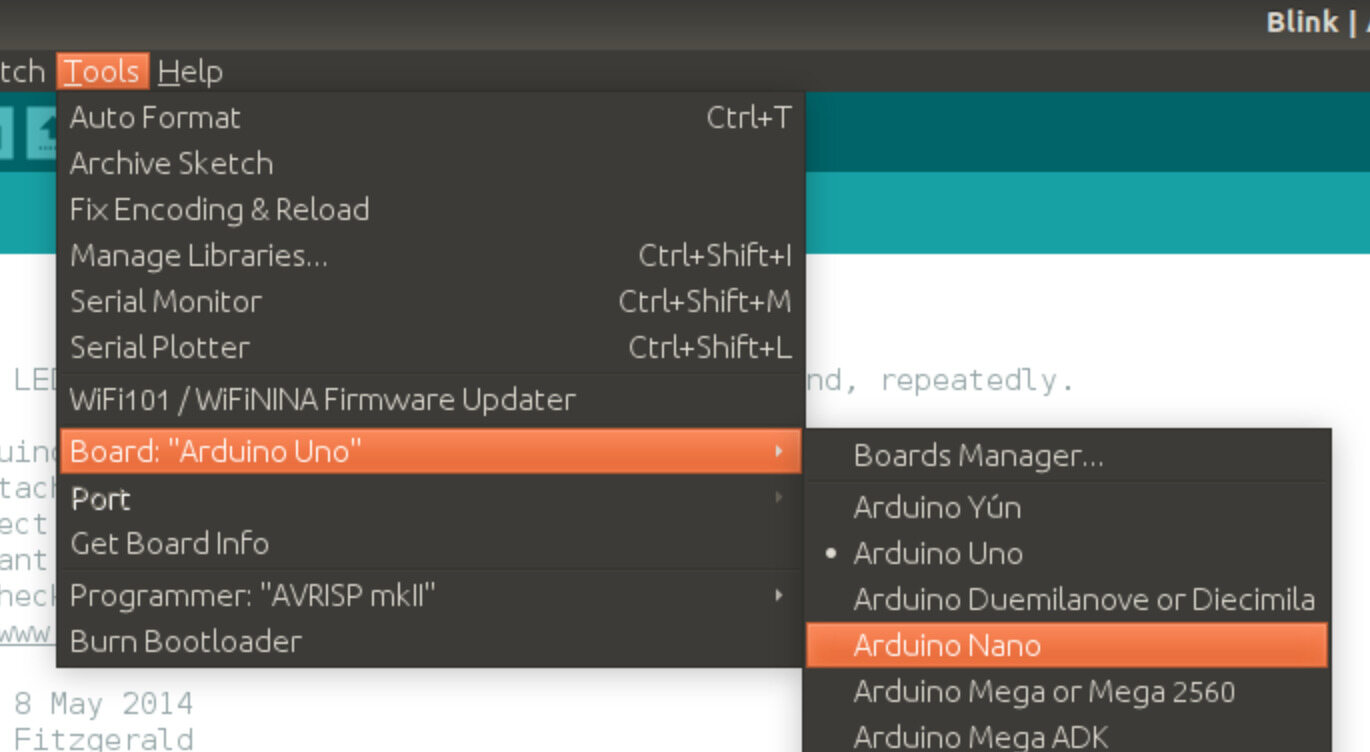
\includegraphics[width=7cm]{microcontroller/ide/selecting-nano-1_8}
%        \label{fig:selecting-board-1}
    }
    \hfil
    \subfloat[Selecting the board with Arduino IDE 2.0.] {
    % 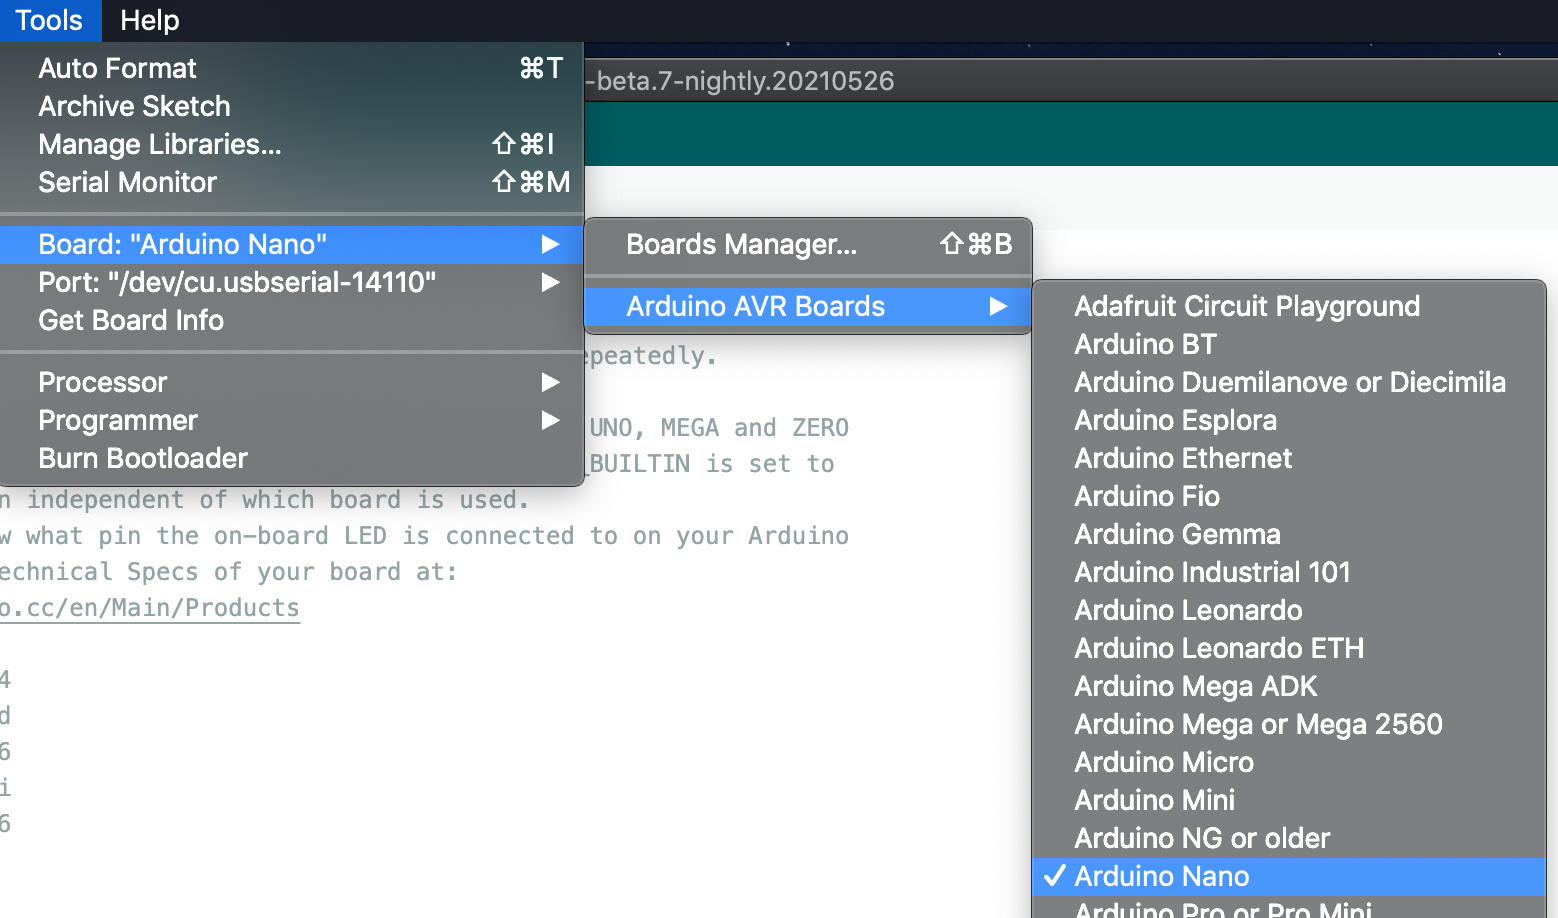
\includegraphics[width=7cm]{selecting-nano-from-menu}
        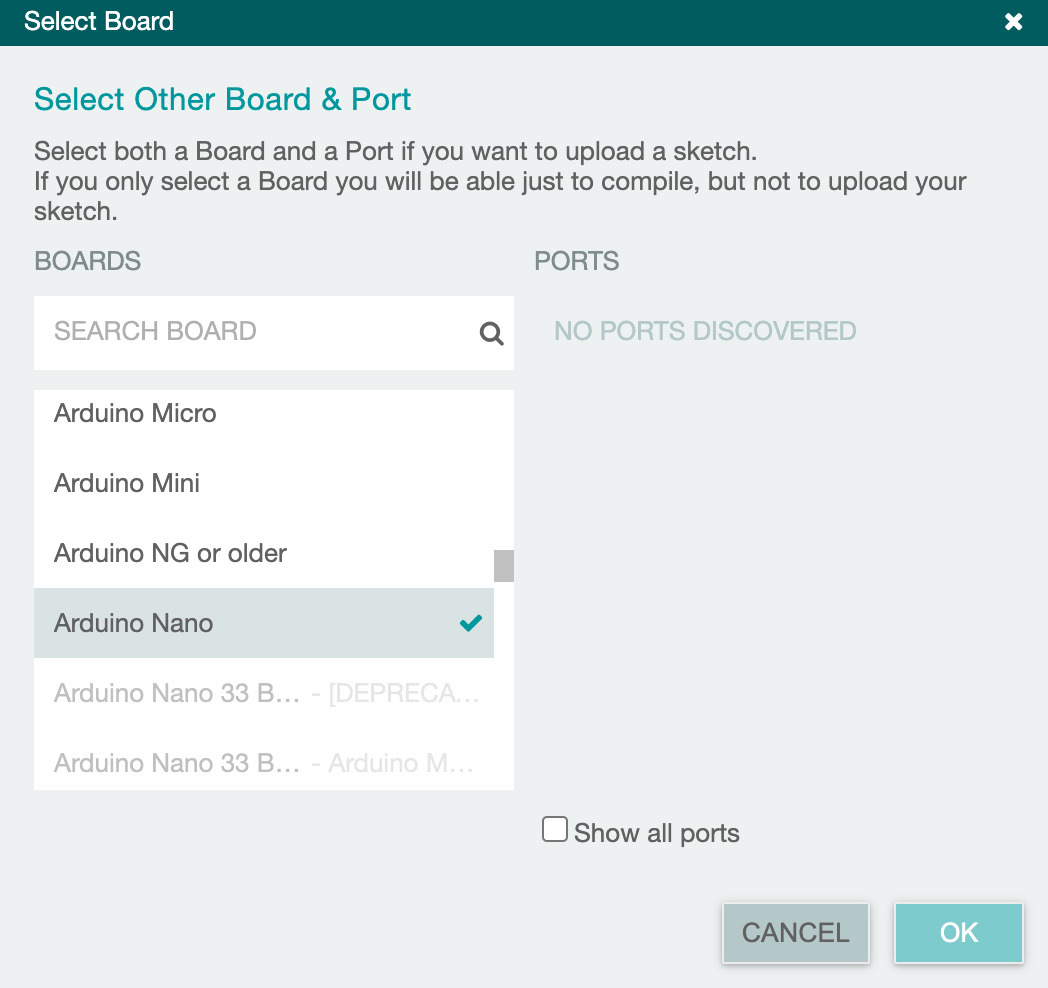
\includegraphics[height=4.1cm]{microcontroller/ide/selecting-nano}
%        \label{fig:selecting-board-2}
    }

    \subfloat[Selecting the processor after selecting the board.] {
    % \vtop{\vskip-4.1cm\hbox{\includegraphics[width=5cm]{selecting-nano-processor}}}
        \includegraphics[width=7cm]{microcontroller/ide/selecting-nano-processor}
        \label{fig:selecting-processor}
    }
    \caption{Selecting board and processor in the Arduino IDE.
    \label{fig:selecting-mcu}}
\end{figure}

\subsubsection{Selecting the Correct ``Processor''}\label{subsubsec:processor-selection}

There are \textit{three} choices for the \developmentboard{}'s processor, two of which specify the ATmega328P processor.
Even though the difference is a USB interface issue, it is resolved through the Arduino IDE's ``Processor'' selection:

\begin{itemize}
    \item Official \developmentboard{}s use the FT232RL USB interface chip.
    Under the ``Tools'' menu, when choosing ``Processor'', select ``ATmega328P''.
    \item \textit{Most} \developmentboard\ clones use the CH340 USB interface chip.
    Under the ``Tools'' menu, when choosing ``Processor'', select ``ATmega328P (Old Bootloader)''.
    (If you are using the Arduino IDE 1.8.4 and earlier, which don't have the ``(Old Bootloader)'' option, simply select ``ATmega328P'').
    \item If you have an older \developmentboard\ that the ATmega168 processor, replace it with one that has an ATmega328P processor.
\end{itemize}

\subsubsection{Updating USB Driver if Necessary}

We have seen some Windows computers without the CH340 USB driver.
If you encounter this problem and the Device Manager shows you the warning in Figure~\ref{fig:usb-warning}, then the first thing to try is updating the driver.
Right-click on USB2.0-Seri! (Figure~\ref{fig:update-driver}) and choose ``Update driver''.
Then choose ``Search automatically for updated driver software''.

\begin{figure}
    \centering
    \subfloat[] {
        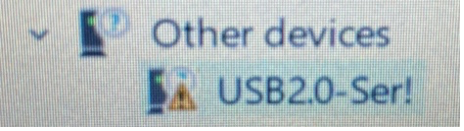
\includegraphics[width=.4\textwidth]{microcontroller/usb-drivers/device-manager-warning}
        \label{fig:usb-warning}
    }
    \hfil
    \subfloat[] {
        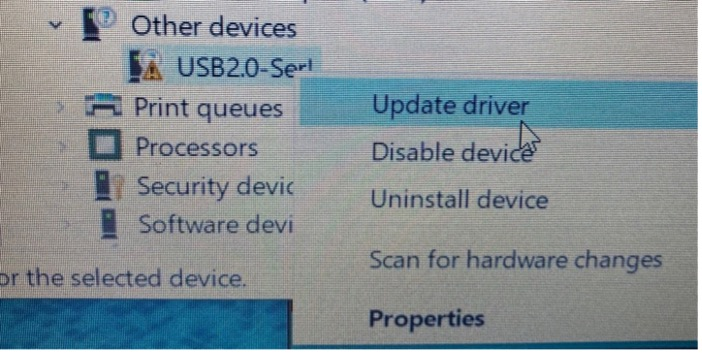
\includegraphics[width=.4\textwidth]{microcontroller/usb-drivers/update-driver}
        \label{fig:update-driver}
    }
    \caption{Selecting board and processor in the Arduino IDE.}
\end{figure}

If Windows reports that ``Windows has successfully updated your drivers'' then you should now be able to connect to the \developmentboard.
On the other hand, if Windows reports that ``Windows was unable to install your USB2.0-Ser!'', then the \href{https://learn.sparkfun.com/tutorials/how-to-install-ch340-drivers/}{How to Install CH340 Drivers} page at sparkfun.com will guide you through manually downloading the driver and installing it.

Sparkfun's \href{https://learn.sparkfun.com/tutorials/how-to-install-ch340-drivers/}{How to Install CH340 Drivers} page also has instructions for installing the driver on MacOS and on Linux;
however, we are not aware of any students needing to manually install the CH340 driver on MacOS\@.

\subsubsection{No Driver Warning but Cannot Connect}

Probably what happened is that your computer has the driver, but you're telling the IDE to connect to the wrong virtual COM port.
The typical way to handle this is to disconnect the \developmentboard\ from your computer, go to the part of the menu where you connect to the COM port, connect the \developmentboard\ to your computer, and select whichever COM port appears after plugging in the \developmentboard.


\subsection{Upload a New Sketch}

    \begin{description}
        \checkoffitem{From the Arduino IDE's File menu, open the \textit{Blink.ino} example:} \\
            \textit{File} $\rightarrow$ \textit{Examples} $\rightarrow$ \textit{01.Basics} $\rightarrow$ \textit{Blink} \\
            Select \textit{Save As...} and save the project as \textit{MyBlink}.
        \checkoffitem{Edit the values in the \function{delay} calls to change the delays between the LED turning on, off, and on again.
        Select values that will visibly have a difference, such as 250 or 2000.}
        \checkoffitem{Compile the program using the ``Verify'' checkmark in the IDE's toolbar and make corrections if the program doesn't compile.}
        \checkoffitem{Upload the program to your \developmentboard\ using the ``Upload'' arrow in the IDE's toolbar.
            (If you forget to compile first, the IDE will compile your program before uploading, but I find it useful to find compile-time mistakes before attempting to upload the program.)}
    \end{description}

    If you successfully uploaded \textit{MyBlink.ino} then you will see the following in the IDE's \textit{Output} window:
    \begin{quote}
    \dots (elided configuration data)\dots
    \begin{verbatim}
    avrdude: AVR device initialized and ready to accept instructions

    Reading | ################################################## | 100% 0.01s

    avrdude: Device signature = 0x1e950f (probably m328p)
    avrdude: reading input file "/var/folders/p7/lx4gt70d0_34cpy8r0j3c95c0000gp/T/arduino-sketch-11A4823C54657006C9F78B0812B621A8/MyBlink.ino.hex"
    avrdude: writing flash (932 bytes):

    Writing | ################################################## | 100% 0.33s

    avrdude: 932 bytes of flash written

    avrdude done.  Thank you.


    --------------------------
    upload complete.
    \end{verbatim}\end{quote}
    and then the LED's on-off pattern will change, reflecting the \function{delay} values you assigned (Figure~\ref{fig:myblink}).

    \subsubsection*{Handling Errors}

        If you get an error when attempting to upload a sketch, try these corrective measures:

        \begin{enumerate}
            \item Try selecting ``ATmega328P'' and try selecting ``ATmega328P (Old Bootloader)'' (see Figure~\ref{fig:selecting-processor}).
            \item Try uploading again (if you attempt to upload a sketch too soon after connecting your \developmentboard\ to your computer, the USB interface won't have finished its handshake).
            \item The \href{https://support.arduino.cc/hc/en-us/articles/4401874331410--Error-avrdude-when-uploading}{Troubleshooting Guide} recommends disconnecting your \developmentboard\ and reconnecting it, then selecting whichever COM port appears.
        \end{enumerate}

        If, instead of an error, your IDE ``hangs'' while collecting configuration data, try this corrective measure:

        \begin{itemize}
            \item Press the \texttt{RESET} button in the middle of the \developmentboard; the IDE should begin uploading the sketch after you release the button.
        \end{itemize}

    \begin{figure}
        \centering
        \animategraphics[autoplay,loop,height=4cm]{8}{microcontroller/animations/myblink-}{0}{6}
        \caption{\textit{MyBlink.ino} has a different on-off pattern than \textit{Blink.ino}.\label{fig:myblink}}
    \end{figure}

\checkpoint{uploaded new code to the \developmentboard}


\section{Direct Input/Output Devices}                       \subsection{Connect Power and Ground to Power Bus Strips} %! suppress = MissingImport
The columns marked with red and blue stripes are the power bus strips, also known as the power rails.
You will now provide power to the bus strips so that the other components can use power.

\disconnect\

% TODO: when we introduce 3.3V options, leaving the two wires attached to each other won't work -- consider changing it now
% TODO: generify pins and contact points
Take the \rainbow, and peel off two wires together.
In the interest of keeping track of which wires are used for which purposes, it would be best to leave the two wires attached to each other as a 2-conductor cable (Figure~\ref{fig:two-wires}).
At one end of this 2-conductor cable, insert one lead into contact point a12 (notice that contact point a12 is electrically connected to the \developmentboard's \texttt{5V} pin, which is in contact point c12) and the other into contact point A14 (notice that contact point A14 is electrically connected to one of the \developmentboard's \texttt{GND} pins, which is in contact point c14); see Figure~\ref{fig:power-step-1}.
Insert the other end of the \texttt{5V} wire into the lower \power\ marked with a red stripe.
Insert the other end of the \texttt{GND} wire into the lower \ground\ marked with a blue stripe.
\textit{Pay attention to the colors of the wires that you're using, so that you know that you connected the \texttt{5V} and \texttt{GND} pins to the power rails and \underline{not} to each other!}
See Figure~\ref{fig:power-step-2}.

\begin{figure}
    \centering
    \subfloat[]{
        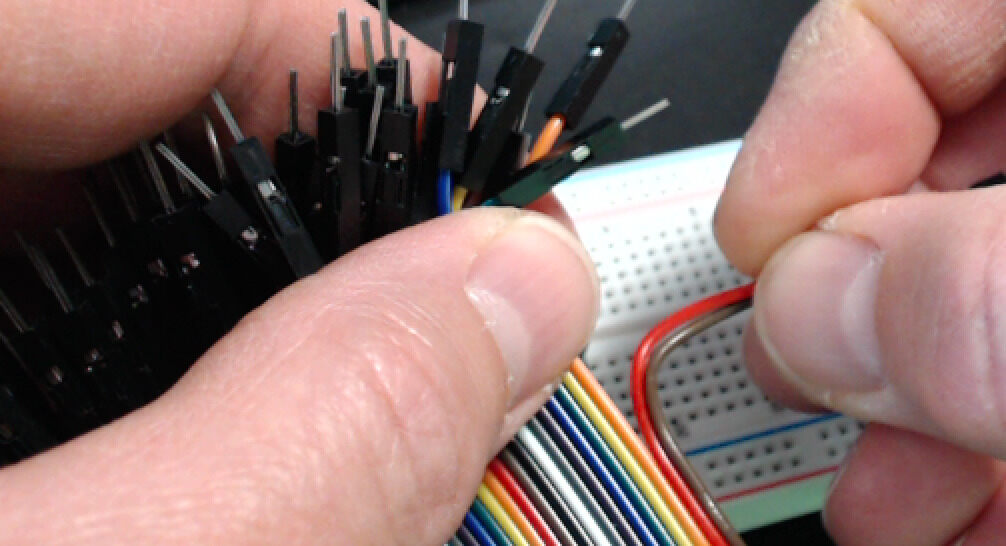
\includegraphics[width=0.4\textwidth]{direct/power/removing-two-wires}
    }
    \hfil
    \subfloat[]{
        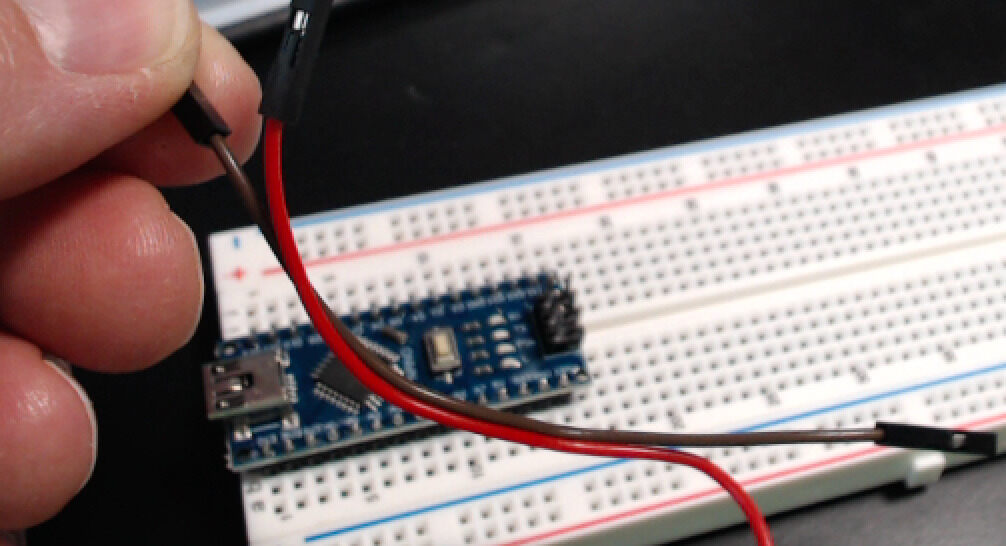
\includegraphics[width=0.4\textwidth]{direct/power/two-wires}
    }
    \caption{Removing a two-conductor cable from the 40-conductor cable.\label{fig:two-wires}}
\end{figure}

\begin{figure}
    \centering
    \subfloat[Tapping power and ground from the \developmentboard.]{
        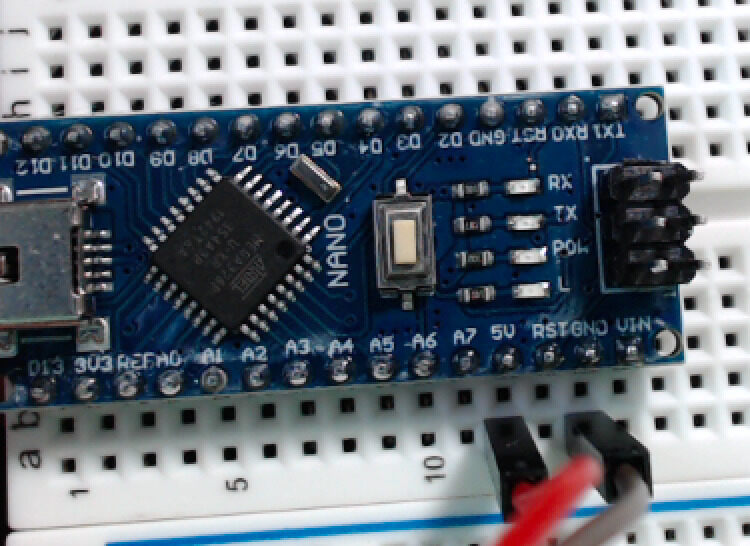
\includegraphics[width=0.27\textwidth]{direct/power/power-step-1}
        \label{fig:power-step-1}
    }
    \hfil
    \subfloat[Connecting lower power bus to power and ground.]{
        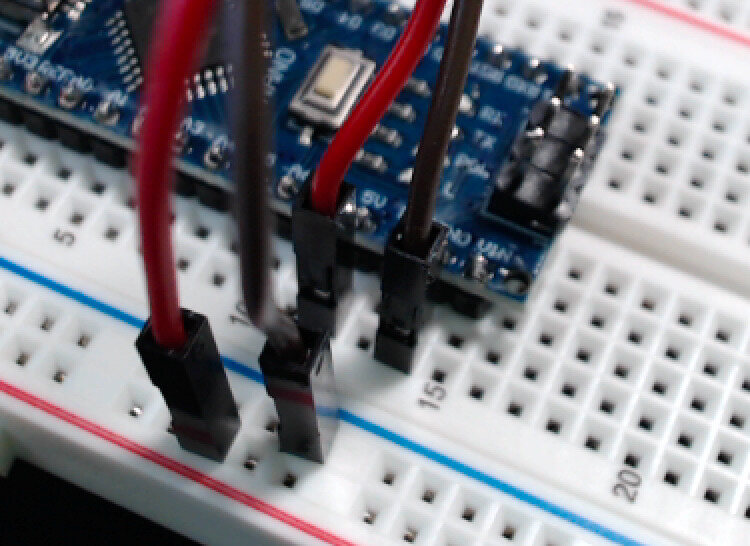
\includegraphics[width=0.27\textwidth]{direct/power/power-step-2}
        \label{fig:power-step-2}
    }
    \hfil
    \subfloat[Connecting upper and lower power busses.]{
        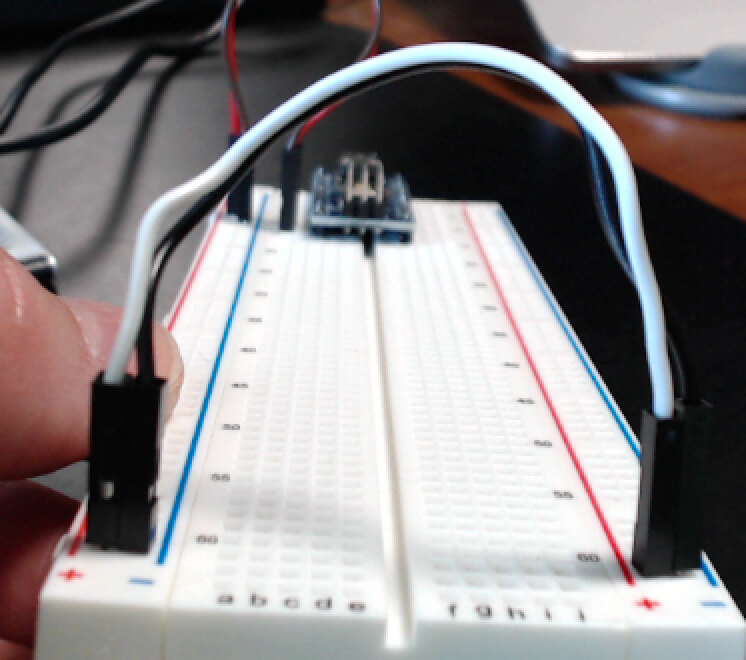
\includegraphics[width=0.27\textwidth]{direct/power/power-step-3}
        \label{fig:power-step-3}
    }
    \caption{Providing power and ground to power busses.}
\end{figure}

Peel off another 2-wire cable from the \rainbow.
Use this 2-conductor cable to connect the lower \power\ to the upper \power, and to connect the lower \ground\ to the upper \ground.
If you place this cable on the right end of the breadboard, it will be out of the way during the remaining steps;
see Figure~\ref{fig:power-step-3}. % TODO: "for now"

\checkpoint{connected the \power{}s and the \ground{}s}


\subsection{Light Emitting Diode} %! suppress = MissingImport
You will now connect an external LED. An LED is a \textit{light emitting diode}, and like all diodes it allows current to flow only in one direction.
As shown in Figure~\ref{fig:led-annotated}, one lead on the LED is longer than the other, and this tells us which direction current will flow.
When we insert the LED into the circuit, power will flow from one of the \developmentboard's pins through the LED to ground.
Most LEDs have so little internal resistance that, unless current is otherwise limited, enough current will flow through the LED to destroy the semiconductor material.
The typical solution, which we will use, is to employ a \textit{current-limiting resistor}.
(If you look very closely at your \developmentboard, you will see a tiny surface-mount resistor next to each built-in LED.)

Figure~\ref{fig:led-diagram} shows a diagram of the components you will install for the LED output.

\begin{figure}
    \centering
    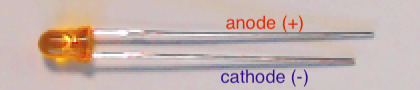
\includegraphics[height=2cm]{direct/led/led-annotated}
    \caption{The LED's longer lead connects to power; the shorter lead connects to ground.\label{fig:led-annotated}}
\end{figure}

\begin{figure}
    \centering
    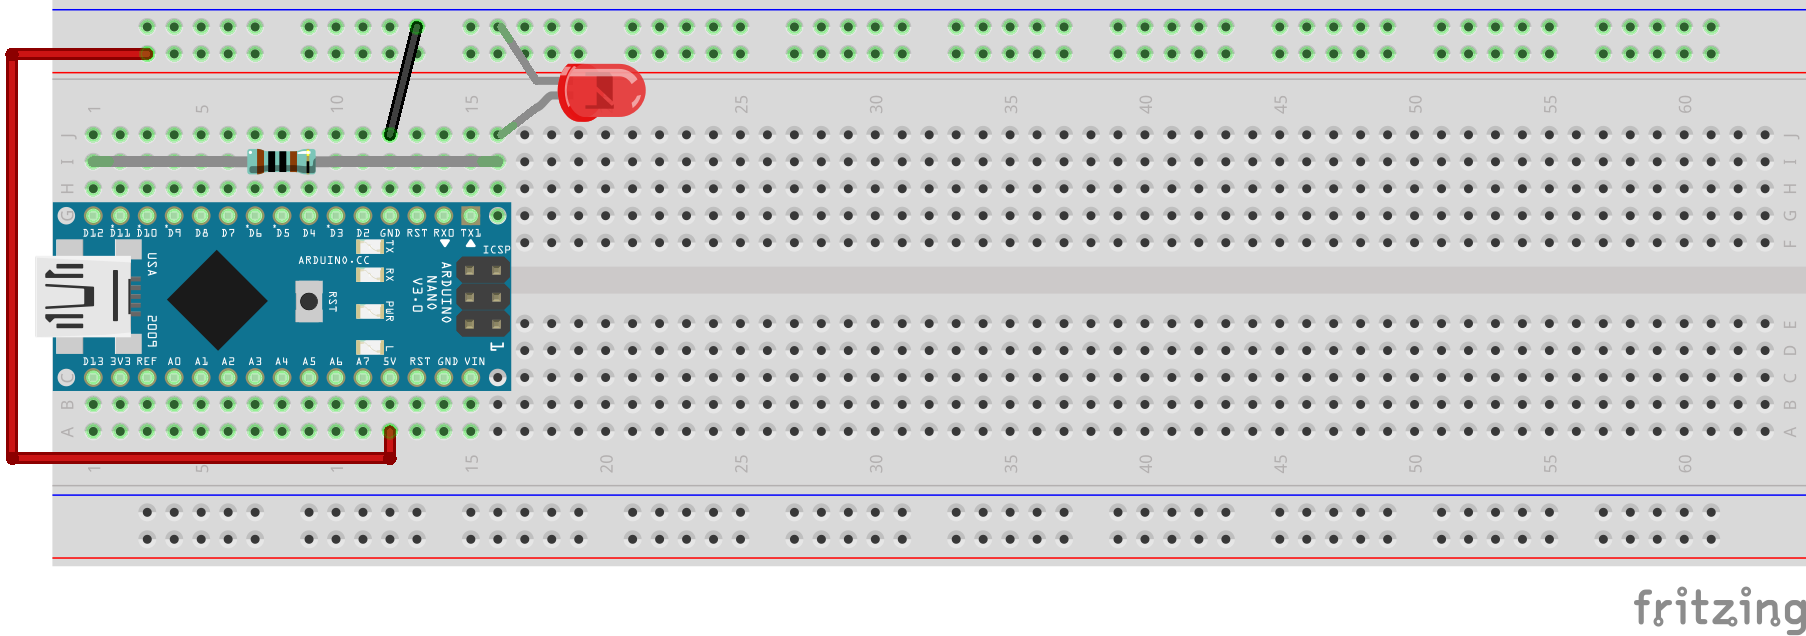
\includegraphics[width=0.9\textwidth]{fritzing_diagrams/led}
    \caption{Diagram of component assembly for LED output. \label{fig:led-diagram}}
\end{figure}

Take the 1k$\Omega$ resistor and place a right-angle bend in each lead about 0.4in (1cm) from the ends (we want the remaining length to be about 1.5in (3.8cm) -- you do not need to be exact;\footnote{If you want to try to be exact, you can use the breadboard's contact points to measure: they are 0.1in (2.54mm) apart.}
the leads are flexible enough that you only need to be approximate) -- see Figure~\ref{fig:resistor-bent}.
Insert one of the resistor's leads into contact point \resistorcontactpointone\ (electrically connected to the \developmentboard's \ledpin\ pin in g1) and the other into contact point \resistorcontactpointtwo.
Gently press along the length of the resistor, causing the leads to deform slightly, until the resistor's height above the breadboard is about the same as the \developmentboard's printed circuit board.
See Figure~\ref{fig:resistor-inserted}.

Take the LED and spread the leads apart slightly.
Insert the longer lead (the anode) in contact point \ledanodecontactpoint, and the shorter lead (the cathode) in the upper \ground.
See Figure~\ref{fig:led-inserted}.

\begin{figure}
    \centering
    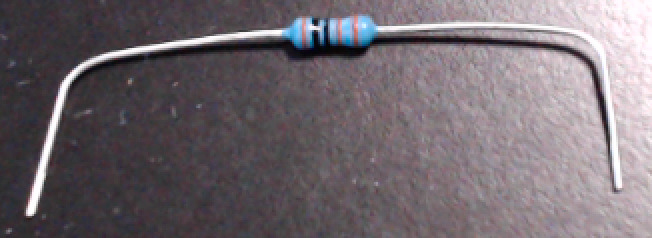
\includegraphics[height=2cm]{direct/led/resistor-bent}
    \caption{Bend the resistor's leads about 1cm from the ends.\label{fig:resistor-bent}}
\end{figure}

\begin{figure}
    \centering
    \subfloat[The resistor run between contact points \resistorcontactpointone\ and \resistorcontactpointtwo.]{
        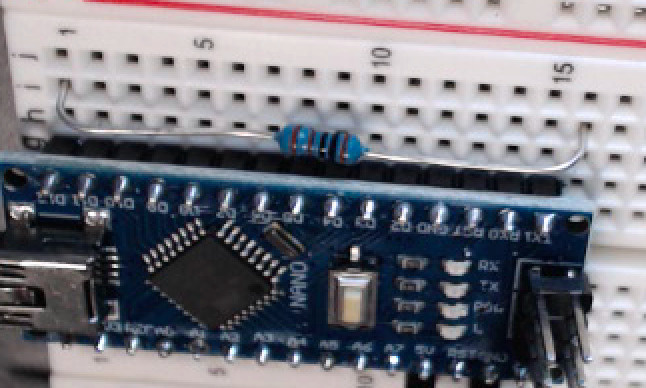
\includegraphics[width=0.65\textwidth]{direct/led/resistor-inserted}
        \label{fig:resistor-inserted}
    }
    \hfil
    \subfloat[The LED's longer lead is in contact point \ledanodecontactpoint, and its shorter lead is in the \ground.]{
        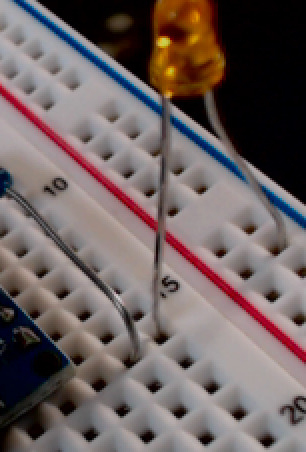
\includegraphics[width=0.25\textwidth]{direct/led/led-inserted}
        \label{fig:led-inserted}
    }
    \caption{Constructing the LED assembly.}
\end{figure}

When you have finished installing the external LED, there should be the electrical connections described in Table~\ref{tab:led}.

\begin{table}
    \begin{center}\begin{tabular}{||c|c|c|c||} \hline\hline
    LED lead    & Resistor lead & \developmentboard\ pin    & Pulled High/Low \\ \hline
    Anode       & Right         &           & \\
    Cathode     &               &           & Pulled Low \\
                & Left          & \ledpin\  & \\ \hline\hline
    \end{tabular}\end{center}
    \caption{Electrical Connections for External LED.\label{tab:led}}
\end{table}

\checkpoint{installed the LED and its current-limiting resistor}

In the Arduino IDE, load \textit{MyBlink.ino}.
%TODO: figure out how to generalize MyBlink
In the \function{pinMode} and the two \function{digitalWrite} calls, replace the \lstinline{LED_BUILTIN} argument with \lstinline{12}:
\begin{lstlisting}
void setup() {
  pinMode(12, OUTPUT);
}

void loop() {
  digitalWrite(12, HIGH);
  delay(250);   // or whatever value you used
  digitalWrite(12, LOW);
  delay(1500);  // or whatever value you used
}
\end{lstlisting}
Re-connect the USB cable to your \developmentboard.
Compile the sketch and upload it to your \developmentboard.
Now, instead of the built-in LED, the external LED that you installed will blink (Figure~\ref{fig:revisedblink}).

\begin{figure}
    \centering
    \animategraphics[autoplay,loop,height=4cm]{8}{direct/animations/revisedblink-}{0}{6}
    \caption{The revised \textit{MyBlink.ino} causes the external LED to blink.\label{fig:revisedblink}}
\end{figure}



\subsection{NAND Gates}\label{subsec:nand} %! suppress = MissingImport
The 74LS20 ``chip'' is an integrated circuit (IC) that holds two 4-input NAND gates.
It is in a \textit{dual inline package} (DIP), and solderless breadboards are designed for the DIP form factor to straddle the breadboard's center divider.
A notch on the left side of the DIP helps us orient the IC; the pins are numbered counter-clockwise from the lower-left to the upper-left (Figure~\ref{fig:nand-annotated}).
The relationship between the 74LS20's pins and the NAND gates' inputs and outputs is shown in Figure~\ref{fig:nand-pinout}.

Figure~\ref{fig:nand-diagram} shows the wiring to install the 74LS20.

\begin{figure}
    \centering
    \subfloat[Pin numbers for the 74LS20.]{
        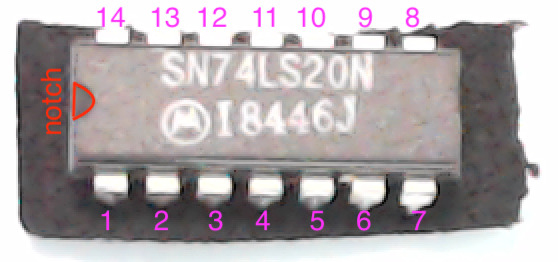
\includegraphics[width=6cm]{direct/nand/nand-annotated}
        \label{fig:nand-annotated}
    }
    \hfil
    \subfloat[Connection diagram showing the 74LS20's pinout.]{
        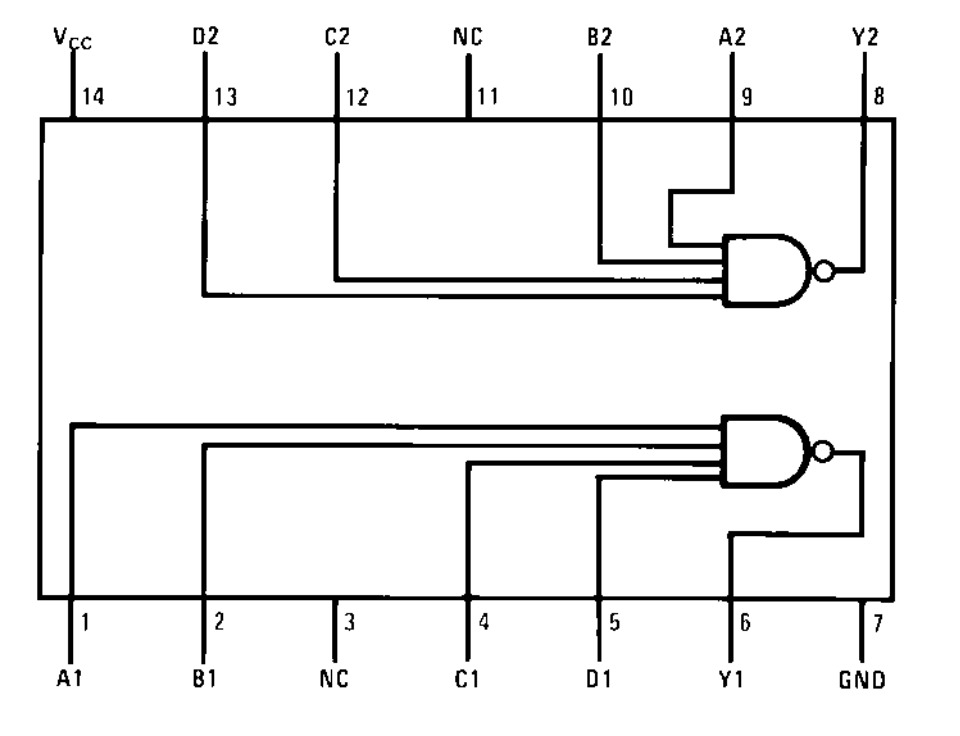
\includegraphics[width=6cm]{direct/nand/nand-pinout}
        \label{fig:nand-pinout}
    }
    \caption{Pin information for the 74LS20.}
\end{figure}

\begin{figure}
    \centering
    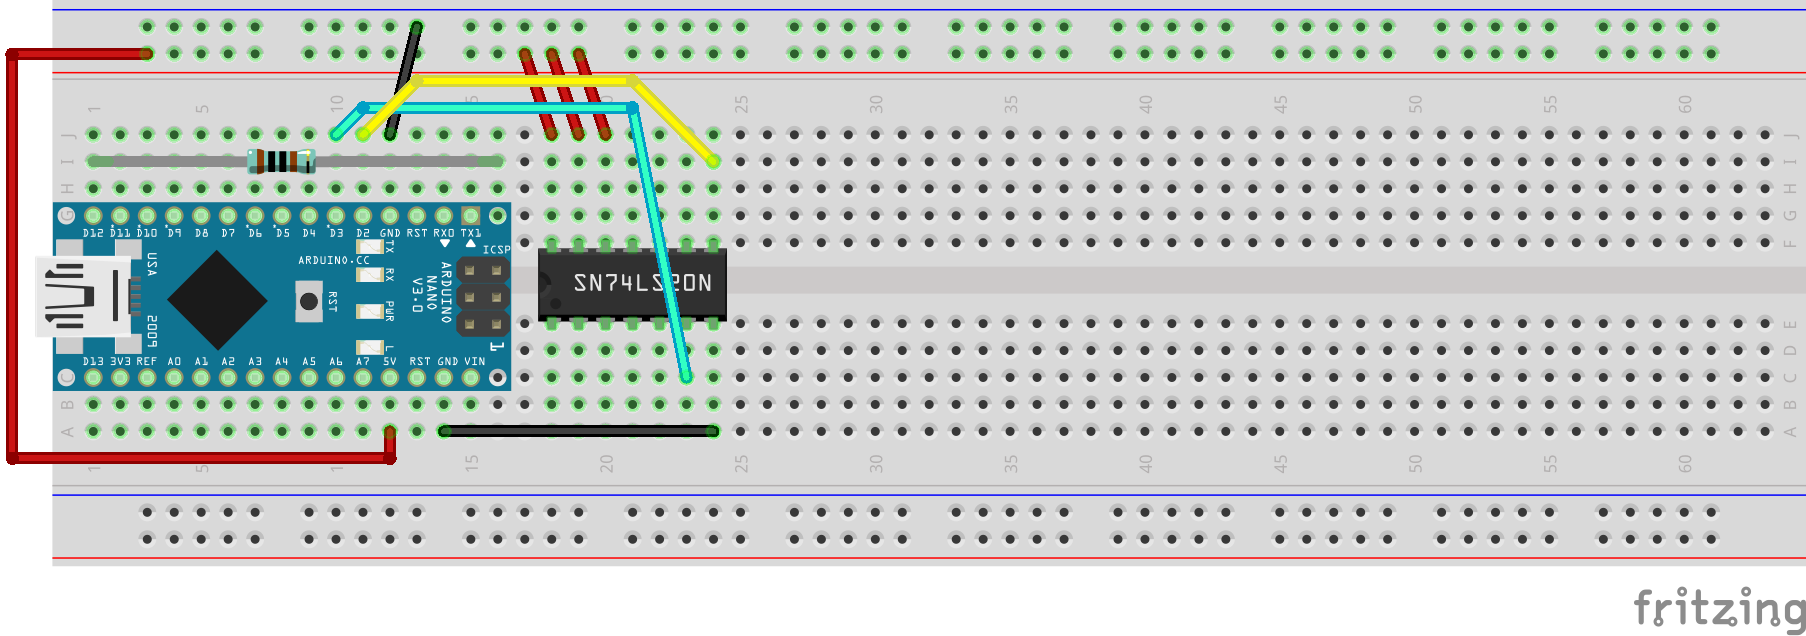
\includegraphics[width=0.9\textwidth]{fritzing_diagrams/nand}
    \caption{Diagram of the 74LS20's installation. \label{fig:nand-diagram}}
\end{figure}

\disconnect\

\begin{description}
    \checkoffitem{\prepunch{\nandupperrow\ and \nandlowerrow}}

    \checkoffitem{Remove the anti-static foam from the 74LS20's pins.}
    \checkoffitem{As described in the \href{https://learn.adafruit.com/breadboards-for-beginners/breadboard-usage}{guide at adafruit.com}, gently press the 74LS20's pins against a tabletop until they're approximately square to the IC's case.}
    \checkoffitem{With its notch to the left, place the 74LS20 on the breadboard straddling the center divider on rows 18--24.}
    \checkoffitem{Double-check that the 74LS20's pins 1--7 are on contact points \nandlowerrow\ and that pins 8--14 are on contact points \nandupperrow\ (Figure~\ref{fig:nand-ready} shows that the IC's pins are not splayed outside the contact points nor are folded under the IC's case).}
    \checkoffitem{Gently press on the 74LS20 to insert the pins into the contact points, using a slight rocking motion if necessary.}
\end{description}
As shown in Figure~\ref{fig:nand-inserted}, the IC is fully inserted when its case is flush with the breadboard.

\begin{figure}
    \centering
    \subfloat[Integrated circuit ready to be inserted.]{
        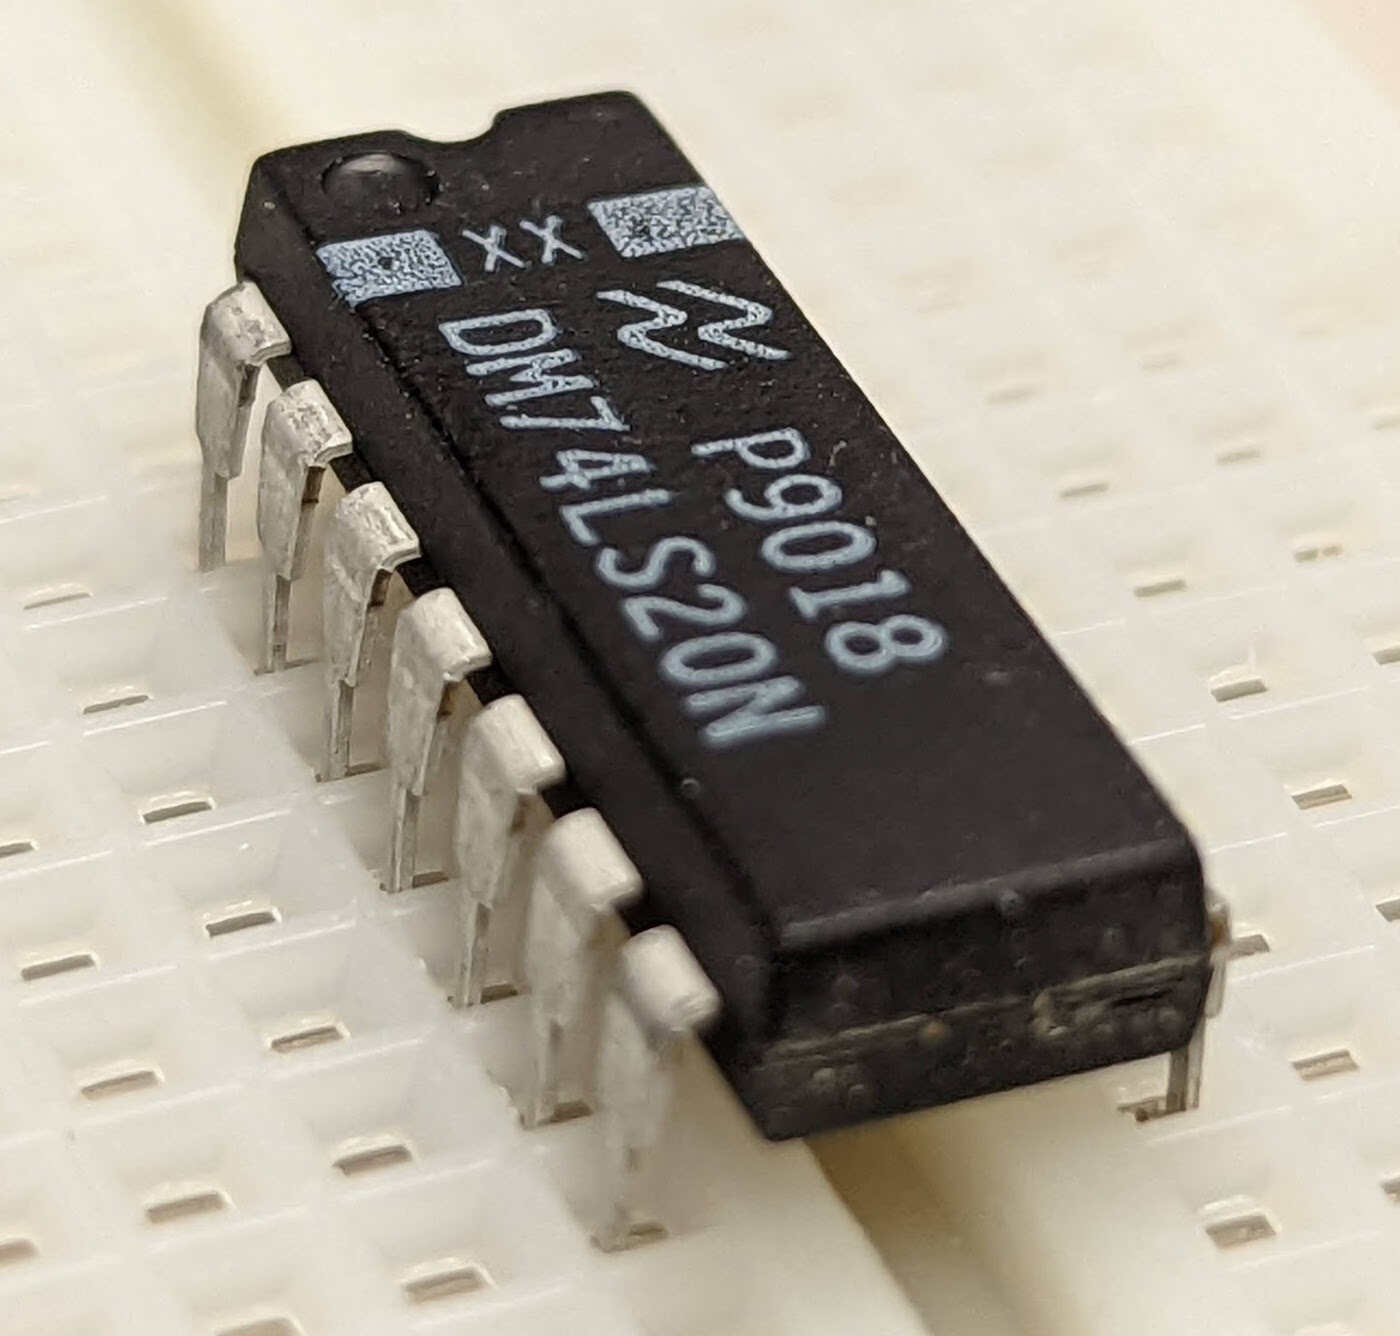
\includegraphics[height=4cm]{direct/nand/nand-ready-to-insert}
        \label{fig:nand-ready}
    }
    \hfil
    \subfloat[Integrated circuit fully inserted.]{
        \includegraphics[height=4cm]{direct/nand/nand-fully-inserted}
        \label{fig:nand-inserted}
    }
    \caption{Inserting the 74LS20.}
\end{figure}

\begin{description}
    \checkoffitem{Peel one wire from the \rainbow;
        use this wire to connect contact point \nandvcc\ (electrically connected to the 74LS20's $\mathtt{V_{CC}}$, pin 14) to the upper \power.}
    \checkoffitem{Peel off another wire from the \rainbow;
        use this wire to connect contact point \nandground\ (electrically connected to the 74LS20's \texttt{GND}, pin 7) to the contact point \mculowergroundcontactpoint\ (electrically connected to one of the \developmentboard's \texttt{GND} pins).
        See Figure~\ref{fig:nand-power}.}

    \checkoffitem{Peel four more wires from the \rainbow.}
    \checkoffitem{Use two wires to connect contact points \nandupperc\ and \nandupperd\ to the upper \power.}
    \checkoffitem{Use another wire to connect contact point \nanduppery\ (electrically connected to the 74LS20's \texttt{Y2}, pin 8) to contact point \mcubuttonnandpoint\ (electrically connected to the \developmentboard's \mcubuttonnand\ pin).}
\end{description}
These three wires configured the 74LS20's upper 4-input NAND gate to act as a 2-input NAND gate;
you will provide the inputs in Section~\ref{subsec:pushbuttons}.
\begin{description}
    \checkoffitem{Use the fourth wire to connect contact point \nandlowery\ (electrically connected to the 74LS20's \texttt{Y1}, pin 6) to contact point \mcukeypadnandpoint\ (electrically connected to the \developmentboard's \mcukeypadnand\ pin).
        See Figure~\ref{fig:nand-outputs}.}
\end{description}
You will provide the inputs for the lower 4-input NAND gate in Section~\ref{sec:keypad}.

\begin{figure}
    \centering
    \subfloat[The 74LS20 connected to power and ground.]{
        \includegraphics[width=.4\textwidth]{direct/nand/nand-power}
        \label{fig:nand-power}
    }
    \hfil
    \subfloat[The 74LS20's outputs connected to the \developmentboard.]{
        \includegraphics[width=.5\textwidth]{direct/nand/nand-outputs}
        \label{fig:nand-outputs}
    }
    \caption{Wiring the 74LS20.}
\end{figure}

When you have finished wiring the 74LS20, there should be the electrical connections described in Table~\ref{tab:nand}.

\begin{table}
    \begin{center}\begin{tabular}{||c|c|c||} \hline\hline
    74LS20 Pin  & \developmentboard\ pin    & Pulled High/Low \\ \hline
    6           & \mcukeypadnand\  & \\
    7           & \multicolumn{2}{c||}{\developmentboard\ \texttt{GND}} \\
    8           & \mcubuttonnand\  & \\
    12          &               & \power\ \\
    13          &               & \power\ \\
    14          &               & \power\ \\ \hline\hline
    \end{tabular}\end{center}
    \caption{Initial Electrical Connections for NAND Gates.\label{tab:nand}}
\end{table}

\checkpoint{inserted and wired the 74LS20}


\subsection{Install the CowPi Library}

\subsection{Slider Switches} %! suppress = MissingImport
In this section, you will install the ``slider'' switches that toggle between their two positions, holding their position until toggled again.
We will wire them such that when a switch is toggled to the left, it will produce a 0, and when it is toggled to the right, it will produce a 1.
Figure~\ref{fig:switch-diagram} shows a diagram of the wiring for the slider switches.

\begin{figure}[p]
    \centering
    \includegraphics[width=0.9\textwidth]{fritzing_diagrams/switch-spi}
    \caption{Diagram of wiring associated with toggle switch input.
        \label{fig:switch-diagram}}
\end{figure}

\disconnect\

Insert one slider switch into contact points a29-a31.
Peel off one wire from the \rainbow, and use it to connect contact point e29 to the upper \ground.
Place the other slider switch into contact points a34-a36.
Peel off another wire from the \rainbow, and use it to connect contact point e34 to the upper \ground.
% See Figure~\ref{fig:switch-power-ground}.

Peel off one wire from the \rainbow, and use it to connect contact point d30 (electrically connected to the left switch's center pin) to contact point a8 (electrically connected to the \developmentboard's \texttt{A4} pin).
Peel off another wire from the \rainbow, and use it to connect contact point d35 (electrically connected to the right switch's center pin) to contact point a9 (electrically connected to the \developmentboard's \texttt{A5} pin).
% See Figure~\ref{fig:switch-nano}. See Figure~\ref{fig:switch-spst}.

The switches' right pins will not be electrically connected to anything.

% \begin{figure}
%     \centering
%     \subfloat[The slider switches, each with their left pin grounded and their
%         right pin connected to 5V.]{
%         \includegraphics[width=0.3\textwidth]{switch-power-ground}
%         \label{fig:switch-power-ground}
%     }
%     \hfil
%     \subfloat[Connections between the \developmentboard\ and the slider switches.]{
%         \includegraphics[width=0.6\textwidth]{switch-nano}
%         \label{fig:switch-nano}
%     }
%     \caption{Wiring the Slider Switches}
% \end{figure}

\begin{figure}
    \centering
    \includegraphics[width=0.6\textwidth]{direct/switches/switch-spst}
    \caption{The slider switches, each with one pin grounded, one pin connected to the \developmentboard, and one pin floating. \label{fig:switch-spst}}
\end{figure}

When you have finished setting up the switches' wiring, there should be the
electrical connections described in Table~\ref{tab:switch}.

\begin{table}
    \begin{center}\begin{tabular}{||c|c|c||} \hline\hline
    Switch                      & \developmentboard\ pin    & Pulled High/Low \\ \hline
    Left switch's left pin      &               & Pulled Low \\
    Left switch's center pin    & \texttt{A4}   & \\
    Left switch's right pin     & \multicolumn{2}{c||}{not connected / floating} \\
    Right switch's left pin     &               & Pulled Low \\
    Right switch's center pin   & \texttt{A5}   & \\
    Right switch's right pin    & \multicolumn{2}{c||}{not connected / floating} \\ \hline\hline
    \end{tabular}\end{center}
    \caption{Electrical Connections for Slider Switches.\label{tab:switch}}
\end{table}

\checkpoint{inserted and wired the slider switches}

Connect your \developmentboard\ to the computer.
In the IDE's Serial Monitor, notice that the LEFT~SWITCH is 0 when the left switch is toggled to the left, and it is 1 when the left switch is toggled to the right.
Similarly, the RIGHT~SWITCH's value is 0 or 1, depending on whether the right switch is toggled to the left or right.

\subsection{Momentary Pushbuttons} %! suppress = MissingImport
This paragraph applies only to 2-lead pushbuttons:
\begin{quote}
    If your momentary pushbuttons are attached to a cardboard strip with tape, remove them from the cardboard strip.
    If your momentary pushbuttons' leads have metal tabs at the end (Figure~\ref{fig:pushbutton-tabs}), you will need to snip off the tabs before inserting the pushbutton leads into the breadboard;
    ordinary scissors will suffice for this task.
    Regardless of whether the leads have metal tabs at the end, you may optionally trim the leads to be about $\frac{1}{4}$in (6.4mm) long -- you can use the exposed lead from a jumper wire as a reference -- so that the pushbuttons sit flush on the breadboard.
    It is not necessary that they sit flush;
    this is simply to keep the buttons from wiggling under your fingers.
    \textit{Do not cut the leads shorter than $\mathit{\frac{1}{8}}$in (3.2mm)!}
    \textbf{Be sure to use eye protection in case the leads' ends fly off when you snip them.}
\end{quote}

This paragraph applies only to 4-prong pushbuttons:
\begin{quote}
    The four prongs on a momentary pushbutton are electrically connected as two pairs.
    If you attach the pushbuttons in the wrong orientation, it will appear to the \developmentboard as though they are always pressed.
    Fortunately, there is only one orientation that will place the prongs in the specified contact points.
    As long as the prongs are in the specified contact points, your pushbuttons will work fine.
    %TODO: add annotated photo of 4-prong electrical connections
\end{quote}

These are ``normally open'' momentary ``switches'' that close when pressed and re-open when released.
We will wire the pushbuttons such that they normally produce a 1, and when pressed will produce a 0.
Figure~\ref{fig:pushbutton-diagram} shows a diagram of the wiring for the pushbuttons.

\begin{figure}
    \centering
    \includegraphics[height=2cm]{direct/buttons/pushbutton-tabs}
    \caption{Some momentary pushbuttons have metal tabs on their leads.\label{fig:pushbutton-tabs}}
\end{figure}

\begin{figure}
    \centering
    \subfloat[2-lead pushbuttons]{
        \includegraphics[width=0.9\textwidth]{fritzing_diagrams/pushbutton-2lead}
    }
    \hfil
    \subfloat[4-prong pushbuttons]{
        \includegraphics[width=0.9\textwidth]{fritzing_diagrams/pushbutton-4prong}
    }
    \caption{Diagram of wiring associated with momentary pushbutton input.
        \textit{Note: connection between the 74LS20's pin 7 and the \developmentboard's
        \mcubuttonnand\ pin was previously installed in Section~\ref{subsec:nand}.}
        \label{fig:pushbutton-diagram}}
\end{figure}

\disconnect\

\prepunch{a\controlrow{11}, a\controlrow{13}, a\controlrow{15}, and a\controlrow{17}}
If you have 4-prong pushbuttons, then also pre-punch holes into contact points d\controlrow{11}, d\controlrow{13}, d\controlrow{15}, and d\controlrow{17}.

If you have 2-lead pushbuttons:
\begin{quote}
    Insert the leads of one pushbutton into contact points a\controlrow{11} and a\controlrow{13}.
    Insert the leads of the other pushbutton into contact points a\controlrow{15} and a\controlrow{17}.
\end{quote}

If you have 4-prong pushbuttons:
\begin{quote}
    Insert the prongs of one pushbutton into contact points a\controlrow{11}, d\controlrow{11}, a\controlrow{13} and d\controlrow{13}.
    Insert the prongs of the other pushbutton into contact points a\controlrow{15}, d\controlrow{15}, a\controlrow{17} and d\controlrow{17}.
\end{quote}

Peel off one wire from the \rainbow, and use it to connect contact point e\controlrow{13} to the upper \ground.
Peel off one wire from the \rainbow, and use it to connect contact point e\controlrow{17} to the upper \ground.

Use two wires from the \rainbow to connect the ungrounded side of the left pushbutton to the 74LS20 and to the \developmentboard:
connect e\controlrow{11} to \leftbuttontarget, and connect \mculeftbuttonfrom\ to \mculeftbuttonpoint.
Now use another two wires from the \rainbow to connect the ungrounded side of the right pushbutton to the 74LS20 and to the \developmentboard:
connect e\controlrow{15} to \rightbuttontarget, and connect \mcurightbuttonfrom\ to \mcurightbuttonpoint.
\textit{Notice that there are no wires in \nanduppernc} because, as you can see in Figure~\ref{fig:nand-pinout}, the 74LS20's pin 11 is not connected (``NC'') to anything.

See Figure~\ref{fig:pushbutton-wired}.

\begin{figure}%\begin{multicols}{2}
    \centering
    \subfloat[The momentary pushbuttons, wired to the 74LS20 and the \developmentboard.]{
        \includegraphics[height=4cm]{direct/buttons/pushbutton-2lead}
    }
%    \columnbreak
%
%    \subfloat[Connections between the momentary pushbuttons and the 74LS20.]{
%        \includegraphics[width=0.55\textwidth]{direct/buttons/pushbutton-nand}
%        \label{fig:pushbutton-nand}
%    }
%
%    \subfloat[Connections between the \developmentboard\ and wiring to the momentary
%        pushbuttons.]{
%        \includegraphics[width=.55\textwidth]{direct/buttons/pushbutton-nano}
%        \label{fig:pushbutton-nano}
%    }
%    \end{multicols}
    \caption{Wiring the Momentary Pushbuttons.
        \label{fig:pushbutton-wired}}
\end{figure}

When you have finished setting up the pushbuttons' wiring, there should be the electrical paths described in Table~\ref{tab:pushbutton}.

\begin{table}
    \begin{center}\begin{tabular}{||c|c|c|c||} \hline\hline
    Pushbutton                      & 74LS20                & \developmentboard\ pin    & Pulled High/Low \\ \hline
    Left button's grounded lead     &                       &                   & Pulled Low    \\
    Left button's ungrounded lead   & Upper NAND Input      & \mculeftbutton    &               \\
    Right button's grounded lead    &                       &                   & Pulled Low    \\
    Right button's ungrounded lead  & Upper NAND Input      & \mcurightbutton   &               \\
                                    & Upper NAND Input      &                   & Pulled High   \\
                                    & Upper NAND Input      &                   & Pulled High   \\
                                    & Upper NAND Output     & \mcubuttonnand    &               \\ \hline
                                    & pin 11 (\nanduppernc) & \multicolumn{2}{c||}{not connected / floating} \\ \hline\hline
    \end{tabular}\end{center}
    \caption{Electrical Paths for Momentary Pushbuttons.\label{tab:pushbutton}}
\end{table}

\checkpoint{inserted and wired the momentary pushbuttons}

Connect your \developmentboard\ to the computer.
In the IDE's Serial Monitor, notice that Left~button is normally UP, but it becomes DOWN when you press the left button.
Similarly, Right~button is normally UP, but it becomes DOWN when you press the right button.
Notice also that Button~NAND is normally 0, but it becomes 1 whenever you press either button (or both).

Notice that both Left~LED and Right~LED are normally OFF\@.
Position both switches to the right.
Notice than when (and only when) the left button is to the right and you're also pressing the left button, Left~LED becomes ON, and the LED labelled ``L'' on the \developmentboard illuminates.
Similarly, when (and only when) the right button is to the right and you're also pressing the right button, Right~LED becomes ON, and the LED that you installed illuminates.
(There may be a delay of about a half-second between you pressing a button and the LED illuminating, and between you releasing a button and the LED deluminating.
We will look at why this happens and how to prevent it in an upcoming lab.)

\section{Matrix Keypad} \label{sec:keypad}                  %! suppress = MissingImport
%\begin{wrapfigure}{r}{0.3\textwidth}
%    \centering
%    \includegraphics[width=0.25\textwidth]{keypad/keypad-annotated}
%    \caption{The numeric keypad's header has four row pins and four column pins. \label{fig:keypad-annotated}}
%\end{wrapfigure}

Observe that the matrix keypad has sixteen buttons has eight pins in its female connector.
As shown in Figure~\ref{fig:keypad-annotated}, when the keypad is face-up and oriented for reading, the four pins on the left are the \textit{row} pins, and the four pins on the right are the \textit{column} pins.
From left-to-right, we will name these pins \texttt{row1}, \texttt{row4}, \texttt{row7}, \texttt{row*}, \texttt{column1}, \texttt{column2}, \texttt{column3}, \texttt{columnA}.
Figure~\ref{fig:keypad-matrix} shows the membrane contacts and which \developmentboard\ pin will be connected to each keypad pin.

%\begin{wrapfigure}{r}{0.3\textwidth}
%    \centering
%    \includegraphics[width=0.25\textwidth]{keypad/keypad-matrix}
%    \caption{The numeric keypad's underlying contact matrix. \label{fig:keypad-matrix}}
%\end{wrapfigure}

\begin{figure}
    \centering
    \subfloat[Front of matrix keypad.] {
        \includegraphics[height=7cm]{keypad/keypad-annotated}
        \label{fig:keypad-annotated}
    }
    \hfil
    \subfloat[Keypad's underlying contact matrix.] {
        \includegraphics[height=7cm]{keypad/keypad-matrix}
        \label{fig:keypad-matrix}
    }
    \caption{The numeric keypad's header has four row pins and four column pins.}
\end{figure}

Figure~\ref{fig:keypad-diagram} shows a diagram of the wiring for the matrix keypad.

\begin{figure}%[p]
    \centering
    \includegraphics[width=0.9\textwidth]{fritzing_diagrams/keypad}
    \caption{Diagram of wiring associated with matrix keyboard input.
        \textit{Note: connection between the 74LS20's pin 8 and the \developmentboard's
        \texttt{D3} pin was previously installed in Section~\ref{subsec:nand}.}
        \label{fig:keypad-diagram}}
\end{figure}

\disconnect\

\prepunch{j\controlrow{0}--j\controlrow{7}}
If your male-male header strip has more than eight pins, then pre-punch additional holes to the right (j\controlrow{8}, j\controlrow{9}, \dots) as needed.

If your 8-pin male-male header strip is not already inserted into the keypad's female connectors, insert it into the female connectors now.
If your male-male header strip has more than eight pins, position the excess pins to the right of the column pins.
Connect your keypad to your breadboard such that \texttt{row1} is in contact point j\controlrow{0}, and \texttt{columnA} is in contact point j\controlrow{7} (and any unused pins on the male-male header are in contact points j\controlrow{8}, j\controlrow{9}, etc.).
\textbf{NOTE}: if you used 20cm wires to connect your slide-switches and/or pushbuttons to the \developmentboard, then you can use the matrix keypad's ribbon cable to pull these wires away from the circuit, reducing clutter near the controls (Figure~\ref{fig:keypad-pullingwires}).

\begin{figure}
    \centering
    \includegraphics{keypad/keypad-pullingwires}
    \caption{The keypad's ribbon cable can be used to pull long wires out of the way. \label{fig:keypad-pullingwires}}
\end{figure}

Peel off three 4-conductor cables from the \rainbow (Figure~\ref{fig:keypad-cables}).
While you \textit{can} use individual wires, having these 4-conductor cables will simplify keeping track of the wires.

\begin{figure}
    \centering
    \includegraphics{keypad/keypad-cables}
    \caption{Three 4-conductor cables. \label{fig:keypad-cables}}
\end{figure}

Insert one end of one of the 4-conductor cables in contact points h\controlrow{0}--h\controlrow{3}, in the same breadboard rows as the keypad's row pins.
Insert the other end of the cable in contact points \mcukeypadrowonepoint--\mcukeypadrowstarpoint.
You want the \developmentboard's \mcukeypadrowone\ pin to connect to the keypad's \texttt{row1} pin, \mcukeypadrowfour\ to \texttt{row4}, \mcukeypadrowseven\ to \texttt{row7}, and \mcukeypadrowstar\ to \texttt{row*};
you can use the wires' colors to make sure that you do so.

Insert one end of another 4-conductor cable in contact points h\controlrow{4}--h\controlrow{7}, in the same breadboard rows as the keypad's column pins.
Insert the other end of the cable in contact points \nandlowerain, \nandlowerbin, \nandlowercin, and \nandlowerdin\ (electrically connected to the 74LS20's \texttt{A1}, \texttt{B1}, \texttt{C1}, and \texttt{D1}: pins 1, 2, 4, and 5).
\textit{Notice that there are no wires in \nandlowernc} because, as you can see in Figure~\ref{fig:nand-pinout}, the 74LS20's pin 3 is not connected (``NC'') to anything.

Insert one end of the remaining 4-conductor cable in contact points \nandloweraout, \nandlowerbout, \nandlowercout, and \nandlowerdout.
Insert the other end in contact points \mcukeypadcolonepoint--\mcukeypadcolApoint\ (electrically connected to the \developmentboard's \mcukeypadcolone--\mcukeypadcolA\ pins).
You want the 74LS20's pin 1 to connect the \developmentboard's \mcukeypadcolone\ pin and the keypad's \texttt{column1} pin, the 74LS20's pin 2 to connect \mcukeypadcoltwo\ and \texttt{column2}, the 74LS20's pin 4 to connect \mcukeypadcolthree\ and \texttt{column3}, and the 74LS20's pin 5 to connect \mcukeypadcolA\ and \texttt{columnA};
you can use the wires' colors to make sure that you do so.

%\begin{figure}
%    \centering
%    \subfloat[The matrix keypad's connector, with the male-male header strip, just before being inserted into the breadboard.
%        Note the excess header strip's excess pin to the right of the column pins, in contact point j34.]{
%        \includegraphics[width=.5\textwidth]{keypad/keypad-header}
%        \label{fig:keypad-header}
%    }
%    \hfil
%    \subfloat[One end of the ``rows'' cable electrically connected to the keypad's row pins.]{
%        \includegraphics[width=.4\textwidth]{keypad/keypad-row-cable}
%        \label{fig:keypad-row-cable}
%    }
%
%    \subfloat[The other end of the ``rows'' cable electrically connected to the \developmentboard's \texttt{D4}-\texttt{D7} pins.]{
%        \includegraphics[width=.4\textwidth]{keypad/keypad-row-nano}
%        \label{fig:keypad-row-nano}
%    }
%    \hfil
%    \subfloat[Connection between the keypad's row pins and the \developmentboard's
%        \texttt{D4}-\texttt{D7} pins.]{
%        \includegraphics[width=.5\textwidth]{keypad/keypad-row-full}
%        \label{fig:keypad-row-full}
%    }
%
%    \subfloat[Connection between the keypad's column pins and the 74LS20.]{
%        \includegraphics[width=.4\textwidth]{keypad/keypad-col-nand}
%        \label{fig:keypad-col-nand}
%    }
%    \hfil
%    \subfloat[Connection between the the 74LS20 and the \developmentboard's \texttt{A0}-\texttt{A3} pins.]{
%        \includegraphics[width=.5\textwidth]{keypad/keypad-col-nano}
%        \label{fig:keypad-col-nano}
%    }
%    \caption{Wiring the Matrix Keypad.}
%\end{figure}

When you have finished setting up the keypad wiring, there should be the electrical paths described in Table~\ref{tab:keypad}.

\begin{table}
    \begin{center}\begin{tabular}{||c|c|c||} \hline\hline
    Keypad pin          & 74LS20            & \developmentboard\ pin \\ \hline
    \texttt{row1}       &                   & \mcukeypadrowone      \\
    \texttt{row4}       &                   & \mcukeypadrowfour     \\
    \texttt{row7}       &                   & \mcukeypadrowseven    \\
    \texttt{row*}       &                   & \mcukeypadrowstar     \\
    \texttt{column1}    & Lower NAND Input  & \mcukeypadcolone      \\
    \texttt{column2}    & Lower NAND Input  & \mcukeypadcoltwo      \\
    \texttt{column3}    & Lower NAND Input  & \mcukeypadcolthree    \\
    \texttt{columnA}    & Lower NAND Input  & \mcukeypadcolA        \\
                        & Lower NAND Output & \mcukeypadnand        \\ \hline
                        & pin 3 (\nandlowernc) & not connected / floating \\ \hline\hline
    \end{tabular}\end{center}
    \caption{Electrical Paths for Matrix Keypad.\label{tab:keypad}}
\end{table}

\checkpoint{inserted and wired the matrix keypad}

%TODO: update for library examples
In the Arduino IDE, open \textit{InputTest.ino}.
Connect your \developmentboard\ to the computer.
Compile \textit{InputTest.ino} and upload it to your \developmentboard.
Open the IDE's Serial Monitor (\textit{Tools} $\rightarrow$ \textit{Serial Monitor}).
You will see several lines reporting the current value of various inputs. (You will also see the \developmentboard's \texttt{TX} LED blinking as the \developmentboard\ sends these lines to your computer.)
Right now, KEYPAD~COLUMNS is always 1111, and KEYPAD~NAND is always 0.
Notice that when you press 1, 4, 7, or *, KEYPAD~COLUMNS becomes 0111;
similarly, pressing a button in the 2$^{nd}$ column causes KEYPAD~COLUMNS to become 1011;
in the 3$^{rd}$ column, 1101;
and in the A$^{th}$ column, 1110.
Whenever any keypad button is pressed, KEYPAD~NAND becomes 1.
Be sure to test all 16 keys.

\section{Display Module}                                    %! suppress = MissingImport
\subsection{Seven-Segment Display Module}

Examine the 7-segment display module.
Notice that the header has five pins (Figure~\ref{fig:display-module-header}): \texttt{VCC} (common collector voltage), \texttt{GND} (ground), \texttt{DIN} (data in), \texttt{CS} (chip select), and \texttt{CLK} (clock).
When the display module is oriented for viewing, these header pins will be on the left.

Figure~\ref{fig:display-diagram} shows a diagram of the wiring to connect the display module to the breadboard.

\begin{figure}
    \centering
    \includegraphics[width=5cm]{display/display-module-header}
    \caption{The display module's header has five pins.
    \label{fig:display-module-header}}
\end{figure}

\begin{figure}
    \centering
    \includegraphics[width=0.9\textwidth]{fritzing_diagrams/display-max7219}
    \caption{Diagram of display module's connections to the breadboard.
    \label{fig:display-diagram}}
\end{figure}

\disconnect\

Take the 5-conductor female-to-male rainbow cable and attach the five female connectors to the display module's five header pins;
see Figure~\ref{fig:display-module-female-connectors}.

As you insert the male connectors into the breadboard, you may have to partially separate the wires at the male end.
In the interest of keeping track of which wires are used for which purposes, do not fully separate the wires.
Identify the wire that is connected to the display module's \texttt{CLK} pin;
insert the male end of this wire in contact point a1 (electrically connected to the \developmentboard's \texttt{D13} pin in c1); see Figure~\ref{fig:display-module-CLK}.
Insert the male end of the \texttt{CS} wire into contact point j3 (electrically connected to the \developmentboard's \texttt{D10} pin in g3); see Figure~\ref{fig:display-module-CS}.
Insert the male end of the \texttt{DIN} wire into contact point j2 (electrically connected to the \developmentboard's \texttt{D11} pin in g2); see Figure~\ref{fig:display-module-DIN}.
Insert the \texttt{GND} wire into a \ground, and the \texttt{VCC} wire into a \power\ (Figure~\ref{fig:display-module-power}).

\begin{figure}
    \centering
    \subfloat[Connect the female ends of the 5-conductor cable to the display module's header pins (your colors may be different).] {
        \includegraphics[width=0.27\textwidth]{display/display-module-female-connectors}
        \label{fig:display-module-female-connectors}
    }
    \hfil
    \subfloat[The display module's clock will be driven by \texttt{D13}.] {
        \includegraphics[width=0.27\textwidth]{display/display-module-CLK}
        \label{fig:display-module-CLK}
    }
    \hfil
    \subfloat[The display module's chip-select will be driven by
    \texttt{D10}.] {
        \includegraphics[width=0.27\textwidth]{display/display-module-CS}
        \label{fig:display-module-CS}
    }

    \subfloat[The display module's data-in will be driven by \texttt{D11}] {
        \includegraphics[width=0.27\textwidth]{display/display-module-DIN}
        \label{fig:display-module-DIN}
    }
    \hfil
    \subfloat[The display module will be powered by the breadboard's power bus] {
        \includegraphics[width=0.27\textwidth]{display/display-module-power}
        \label{fig:display-module-power}
    }
    \caption{Connecting the Display Module.}
\end{figure}

When you have finished connecting the display module, there should be the electrical connections described in Table~\ref{tab:display}.

\begin{table}
    \begin{center}\begin{tabular}{||c|c|c||} \hline\hline
    Display Module Pin  & \developmentboard\ pin    & Pulled High/Low \\ \hline
    \texttt{CLK}         & \texttt{D13}  & \\
    \texttt{CS}          & \texttt{D10}  & \\
    \texttt{DIN}         & \texttt{D11}  & \\
    \texttt{GND}         &               & Pulled Low \\
    \texttt{VCC}         &               & Pulled High \\ \hline\hline
    \end{tabular}\end{center}
    \caption{Electrical Connections for External LED.\label{tab:display}}
\end{table}

\checkpoint{connected the display module to the breadboard}

In the Arduino IDE, open \textit{DisplayTest.ino}.
Connect your \developmentboard\ to the computer.
Compile \textit{DisplayTest.ino} and upload it to your \developmentboard.
You should see {\dviiseg 8.} move back and forth across the display (Figure~\ref{fig:display-test}).
You may be able to see the \developmentboard's built-in LED blink rapidly: recall that it's connected to pin 13, which is used as the clock signal when the \developmentboard\ sends data to the display module.

\begin{figure}
    \centering
    \animategraphics[autoplay,palindrome,height=5cm]{10}{display/animations/displaytest-}{0}{7}
    \caption{\textit{DisplayTest.ino} illuminates all segments on a digit, one digit at a time. \label{fig:display-test}}
\end{figure}


\section*{Kit Assembly is Complete}

    You have now finished assembling the class kit (Figure~\ref{fig:complete}).
    In the upcoming I/O labs, you will use the kit to learn about memory-mapped I/O and about handling low-level interrupts.

\begin{figure}
    \centering
    %! suppress = NonMatchingIf
    \ifdefstring{\serialprotocol}{SPI}{
            \subfloat[]{
                \includegraphics[height=0.55\textheight]{fritzing_diagrams/complete-max7219}
    %            \label{fig:complete-diagram}
            }

            \subfloat[]{
                \includegraphics[height=0.35\textheight]{completed-kit-max7219}
    %            \label{fig:complete-kit}
            }
    }{}
    %! suppress = NonMatchingIf
    \ifdefstring{\serialprotocol}{I2C}{
            \subfloat[]{
                \includegraphics[height=0.55\textheight]{fritzing_diagrams/complete-lcd1602}
    %            \label{fig:complete-diagram}
            }

            \subfloat[]{
                \includegraphics[height=0.35\textheight]{completed-kit-lcd1602}
                \label{fig:complete-kit}
            }
    }{}
\caption{The fully-assembled class kit.\label{fig:complete}}
\end{figure}

\section{Turn-in and Grading}

    When you have completed this assignment, upload \textit{checkpoints.txt} to \filesubmission.

    This assignment is worth 1 point, with up to 5 bonus points for helping other students. \\

    Rubric:
    \begin{description}
        \rubricitem{0.5}{You bring your fully-assembled class kit to your lab section the week it is due.}
        \rubricitem{0.5}{You upload the completed \textit{checkpoints.txt} file to \filesubmission.}
        \bonusitem{0.1}{For each checkpoint you verify for fellow students, as reported in their \textit{checkpoints.txt} files;
            maximum of 5.0 bonus points.}
    \end{description}

\end{document}
